\chapter{Implementierung}
\label{chap:Implementierung}

\section{Editor}
\label{sec:Editor}
Der Editor ist die Schnittstelle zwischen der DSL und einem menschlichen Benutzer. Hier wird ein DSL-Modell durch Interaktion mit der konkreten Syntax erstellt oder bearbeitet. Die konkrete Syntax nimmt die Form des Ablaufdiagramms an, das in Kapitel \ref{chap:Einleitung} beschrieben ist. Mit dem Editor kann dieses Diagramm über die grafische Benutzeroberfläche in die gewünschte Form gebracht werden. Abbildung \ref{fig:EditorGUI} zeigt und erklärt die Komponenten der grafischen Benutzeroberfläche.

\begin{figure} %[hbtp]
	\centering
		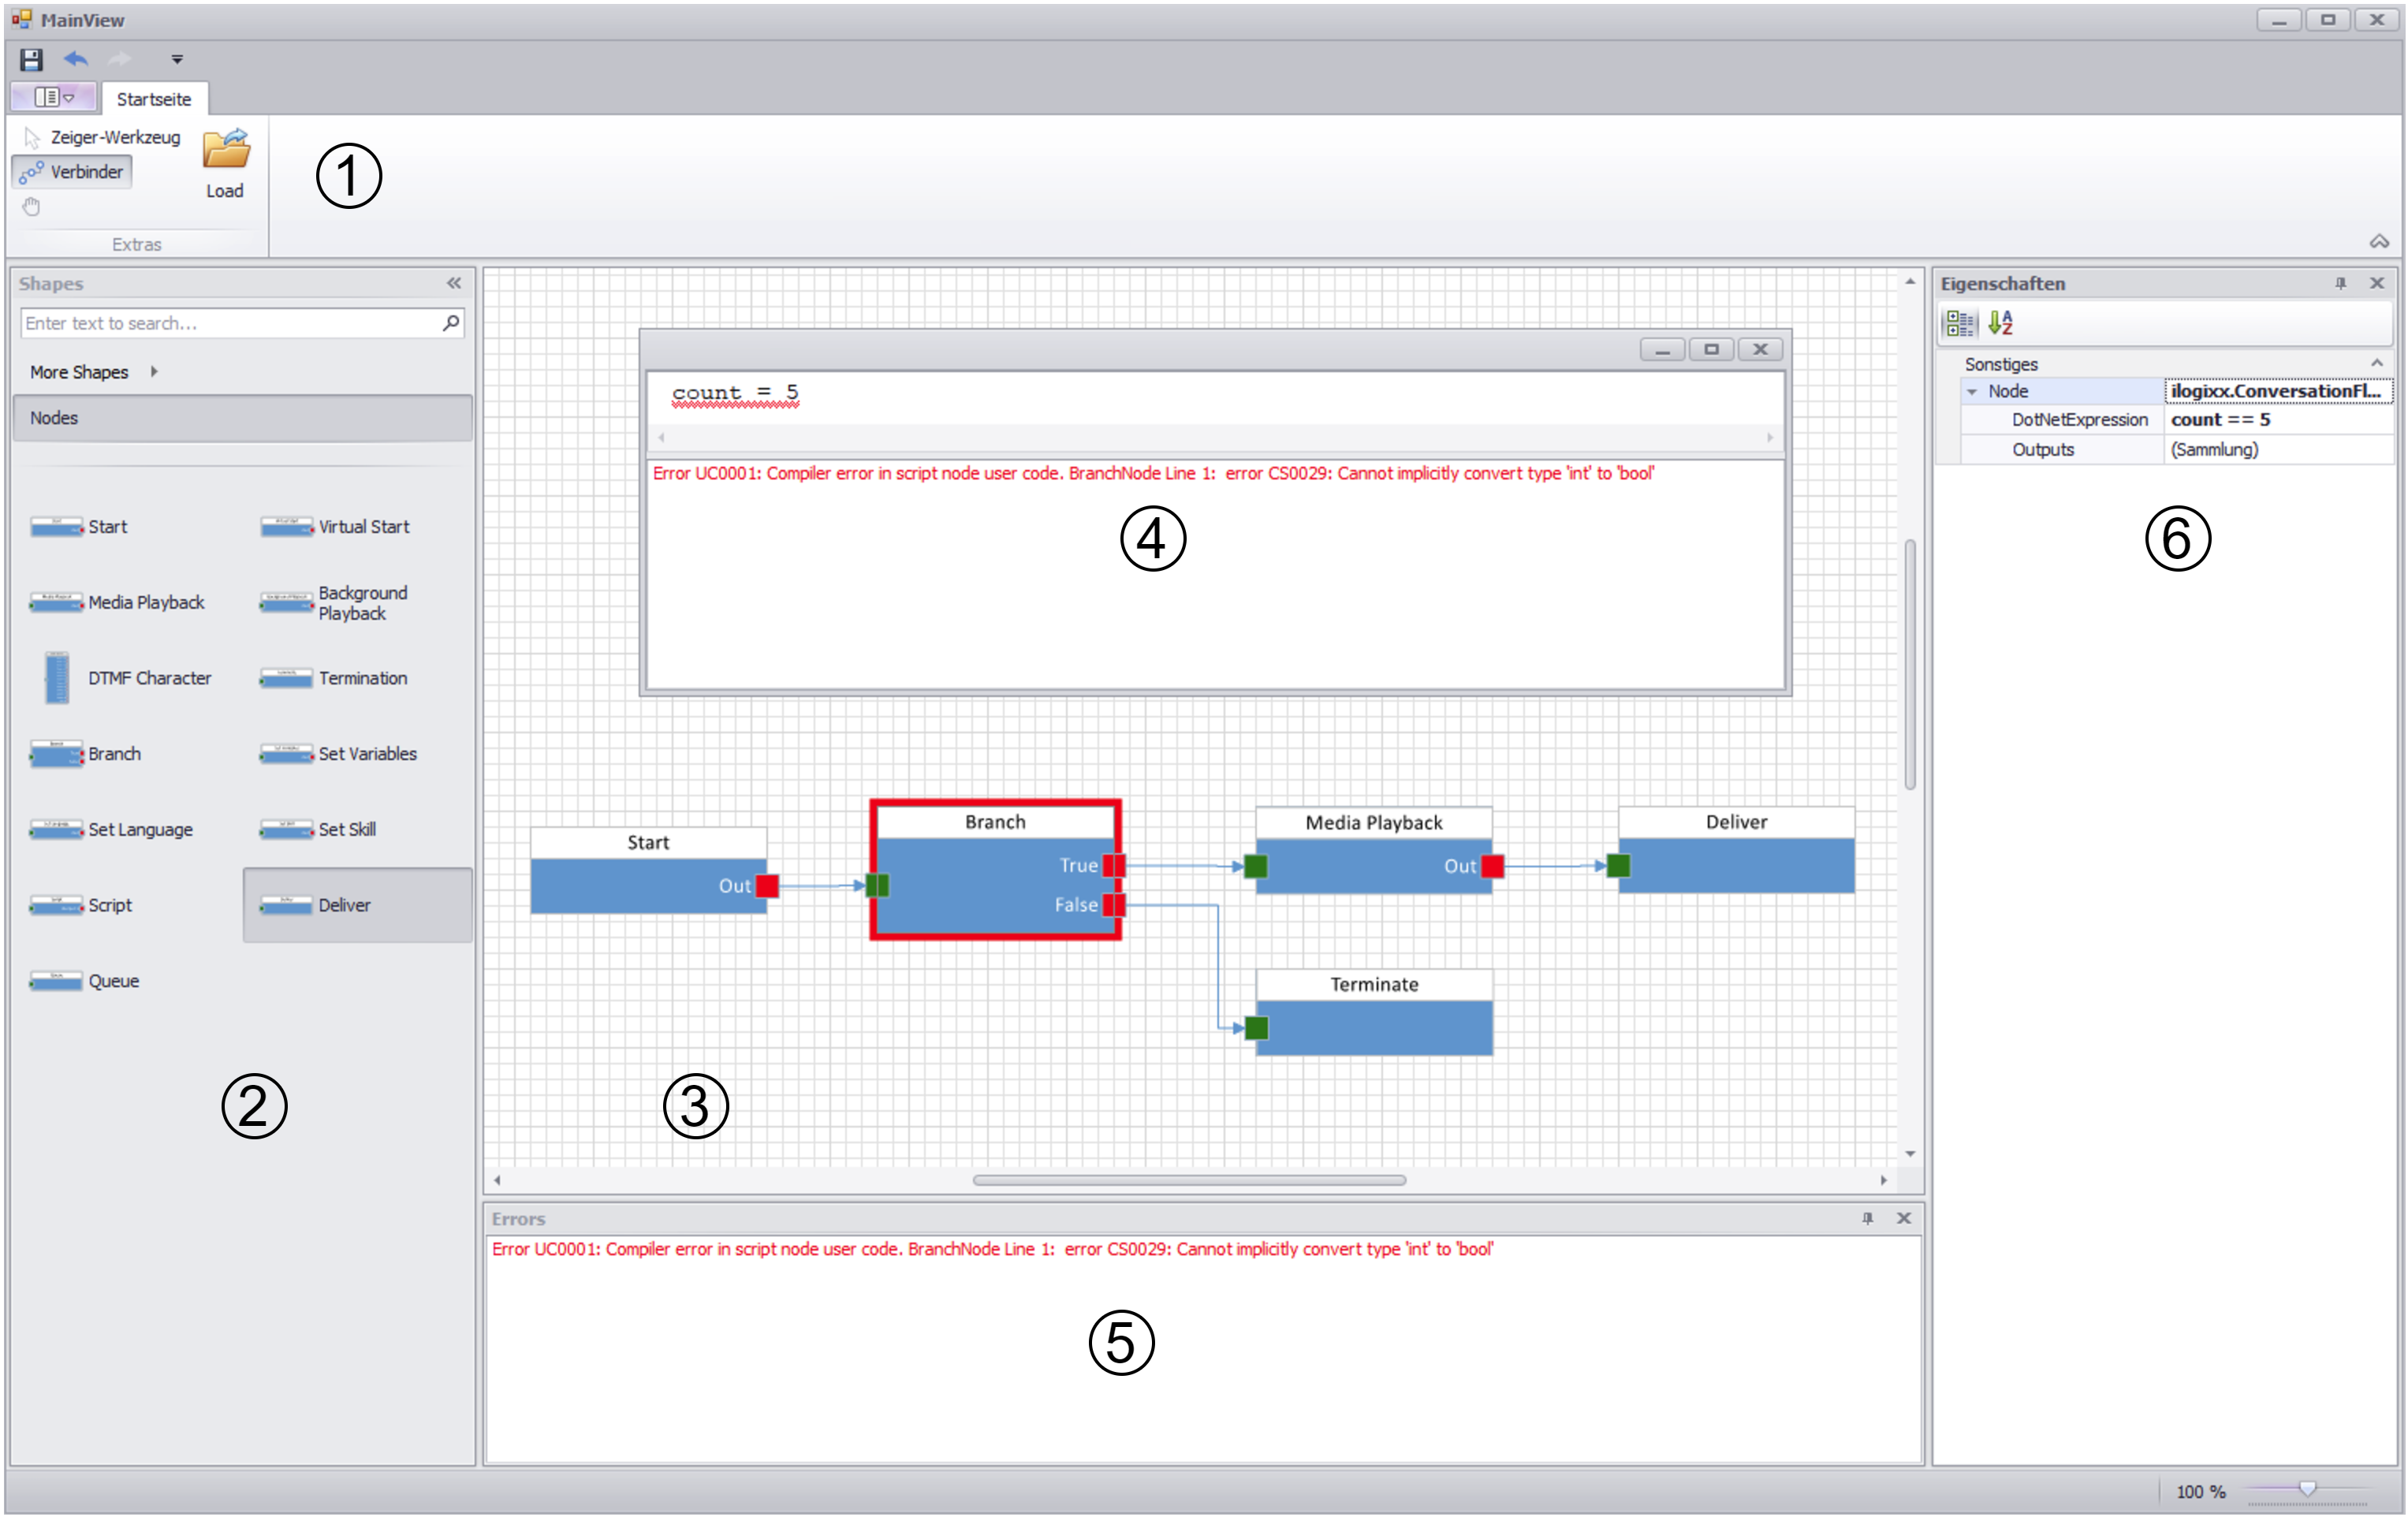
\includegraphics[width=\textwidth]{img/EditorGUI.png}
    \captionsetup{singlelinecheck=off}
	\caption[Die Benutzeroberfläche des Editors]
	{
	\label{fig:EditorGUI}
	\textit{Zu sehen ist die Benutzeroberfläche des Editors. Die Nummerierung beziffert folgende Komponenten:
	\begin{enumerate}
	\item Menüleiste. Hier kann der Benutzer Routings speichern oder laden, sowie das Verbindungswerkzeug zum Verbinden von zwei Instruktionen an- und ausschalten.
	\item Instruktionsauswahl-Fenster. Der Benutzer sieht hier eine Übersicht der verfügbaren Instruktionen. Per "Drag and Drop'' kann er eine Instruktion auswählen und in das Editor-Fenster ziehen.
	\item Editor-Fenster. Hier kann der Benutzer das Konversationsrouting modellieren, indem er Instruktionen hinzufügt, löscht, anordnet und miteinander verbindet.
	\item Ausdruck-Editor. Der Editor ist in dieser Darstellung stellvertretend für alle Editoren dargestellt, die sich in einem weiteren Fenster öffnen. In diesem Fall ist der Ausdruck-Editor geöffnet, da momentan der boolesche Ausdruck für die Branch-Instruktion editiert wird. Hier kann der Benutzer seinen eigenen Code schreiben. Der Editor verfügt über ein eigenes Diagnose-Fenster, in dem Fehlermeldungen dargestellt werden, die sich auf den zu editierenden Code beziehen.
	\item Diagnose-Fenster. Hier werden alle Fehlermeldungen aufgelistet, die durch die Modell-Validierung detektiert werden. Bei Fehlermeldungen, die sich explizit auf eine Instruktion beziehen, werden diese Instruktionen rot umrandet. Durch einen Doppelklick auf eine Fehlermeldung wird die betroffene Instruktion ausgewählt, oder falls nötig, ein Editor geöffnet der den fehlerhaften Code darstellt.
	\item Parameter-Fenster. Hier können die Parameter der aktuell ausgewählten Instruktion angepasst werden. Ist keine Instruktion ausgewählt, können die weiteren Eigenschaften des Konversationsroutings eingestellt werden, wie zum Beispiel benutzerdefinierte Variablen und Funktionen.
 	\end{enumerate}}
 	}
\end{figure}
\noindent Neben der Interaktion mit dem Benutzer ist die andere Aufgabe des Editors, die konkrete Syntax in abstrakte Syntax umzuwandeln. Während der Benutzer über die grafische Benutzeroberfläche mit der konkreten Syntax interagiert, also Instruktionen hinzufügt und Verbindungen zieht, wird Editor-intern die für den Benutzer unsichtbare abstrakte Syntax geformt. Die abstrakte Syntax ist durch die Instanz eines Objekt-Graphen repräsentiert, welcher für die weiteren Verarbeitungsschritte gespeichert wird (siehe Abschnitt \ref{sec:Verarbeitungsschritte}). In der Literatur wird die Datenstruktur, welche die abstrakte Syntax beinhaltet, auch semantisches Modell (engl. semantic model)\cite[S. 159ff]{Fowler:11}, oder abstraktes Syntax-Modell (engl. abstract syntax model)\cite[S. 78ff]{Kleppe:09} genannt. Der Editor bildet eine vom Benutzer modellierte Instanz der konkreten Syntax auf eine Instanz des semantischen Modells ab. Diese Abbildung ist bidirektional: Änderungen am semantischen Modell spiegelt die grafische Benutzeroberfläche in der konkreten Syntax wider. 
\newline
Der Editor ist als eine Windows Forms-Anwendung umgesetzt und implementiert das Model-View-ViewModel-Entwicklungsmuster (kurz MVVM). Ähnlich wie bei verwandten Entwurfsmustern wie zum Beispiel Model-View-Controller (MVC) geht es bei MVVM darum, die Darstellung einer Anwendung von ihrer Logik zu trennen. Dies geschieht durch eine Einteilung in drei verschiedene Schichten: Dem View, dem ViewModel und dem Model. Die View-Schicht dient zur Darstellung der Anwendung und umfasst die Komponenten der grafischen Benutzeroberfläche. Sie erhält die nötigen Daten zur Darstellung vom ViewModel über sogenannte Datenbindung (engl. Data Binding). Dabei werden Daten über ein Framework an einander gebunden und werden so vom System bei jeder Zustandsänderung synchronisiert. Ändern sich also Daten im ViewModel wird dies unverzüglich im View angezeigt. 
\newpage
\noindent Das ViewModel behandelt die Präsentationslogik. Das heißt es ist dafür zuständig Daten so aufzubereiten, dass diese dem View per Datenbindung zur Verfügung gestellt werden können. Dafür hat das ViewModel Zugriff auf das Model, welches die Daten speichert. Im ViewModel wird auch die Geschäftslogik sowie Speicher- und Lade-Aktionen ausgeführt. In .NET wird MVVM vor allem im Zuge der Windows Presentation Foundation eingesetzt, kann aber durch das Devexpress-Framework auch in Windows Forms-Anwendungen benutzt werden. 
\newline
Im grafischen Editor der DSL werden die drei Schichten von MVVM durch verschiedene Klassen abgebildet, welche im Folgenden erläutert werden.

\subsection[Die Model-Schicht]{Die Model-Schicht: Flow, Node, Input, Output, Connector, Variable, Function}
\label{subsec:Die Model-Schicht}
Die Model-Schicht beinhaltet den Objekt-Graphen, welcher auch als semantisches Modell bezeichnet wird. Das semantische Modell selbst weist kein programmatisches Verhalten auf, sondern ist eine reine Datenstruktur. Es besteht aus Instanzen von Klassen, welche die einzelnen Elemente der DSL modellieren und im Namespace ilogixx.ConversationFlow.Core definiert sind. Die Klassenstruktur der Model-Schicht ist in Abbildung \ref{fig:UML:Model-Schicht} als UML-Diagramm aufgeführt.

\begin{figure} %[hbtp]
	\centering
		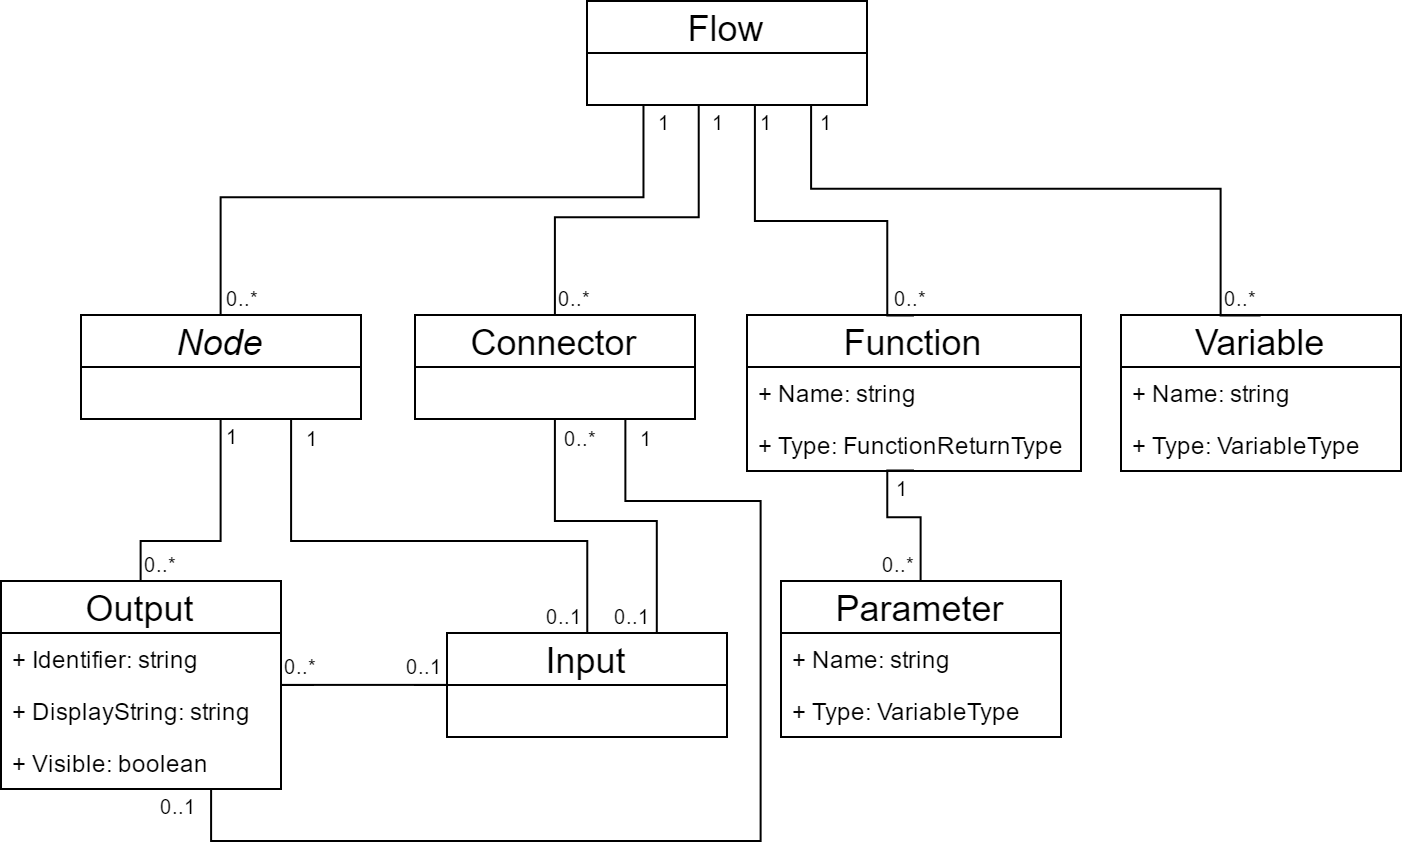
\includegraphics[width=\textwidth]{img/FlowClassStructure.png}
	\caption[Klassenstruktur der Model-Schicht]{\textit{Zu sehen ist ein Teil der Klassenstruktur der Model-Schicht. Diese ist zugleich auch der Objekt-Graph, welcher in folgenden Schritten weiterverarbeitet wird.}}
	\label{fig:UML:Model-Schicht}
\end{figure}
\noindent Das Sprachkonzept einer Instruktion wird auf die abstrakte Klasse \texttt{Node} abgebildet. \texttt{Node} besitzt eine Liste von Referenzen auf \texttt{Output}-Objekte, welche die Ausgänge einer Instruktion modellieren. \texttt{Node} hat ebenfalls eine Referenz auf ein Objekt vom Typ \texttt{Input}, welches den Eingang einer Instruktion symbolisiert. Jede Art von Instruktion aus Abschnitt \ref{subsec:start} bis Abschnitt \ref{subsec:terminate} wird auf ihre jeweils eigene \texttt{Node}-Subklasse abgebildet, dargestellt in Abb. \ref{fig:UML:Node-Hierarchy}.

\begin{figure} %[hbtp]
	\centering
		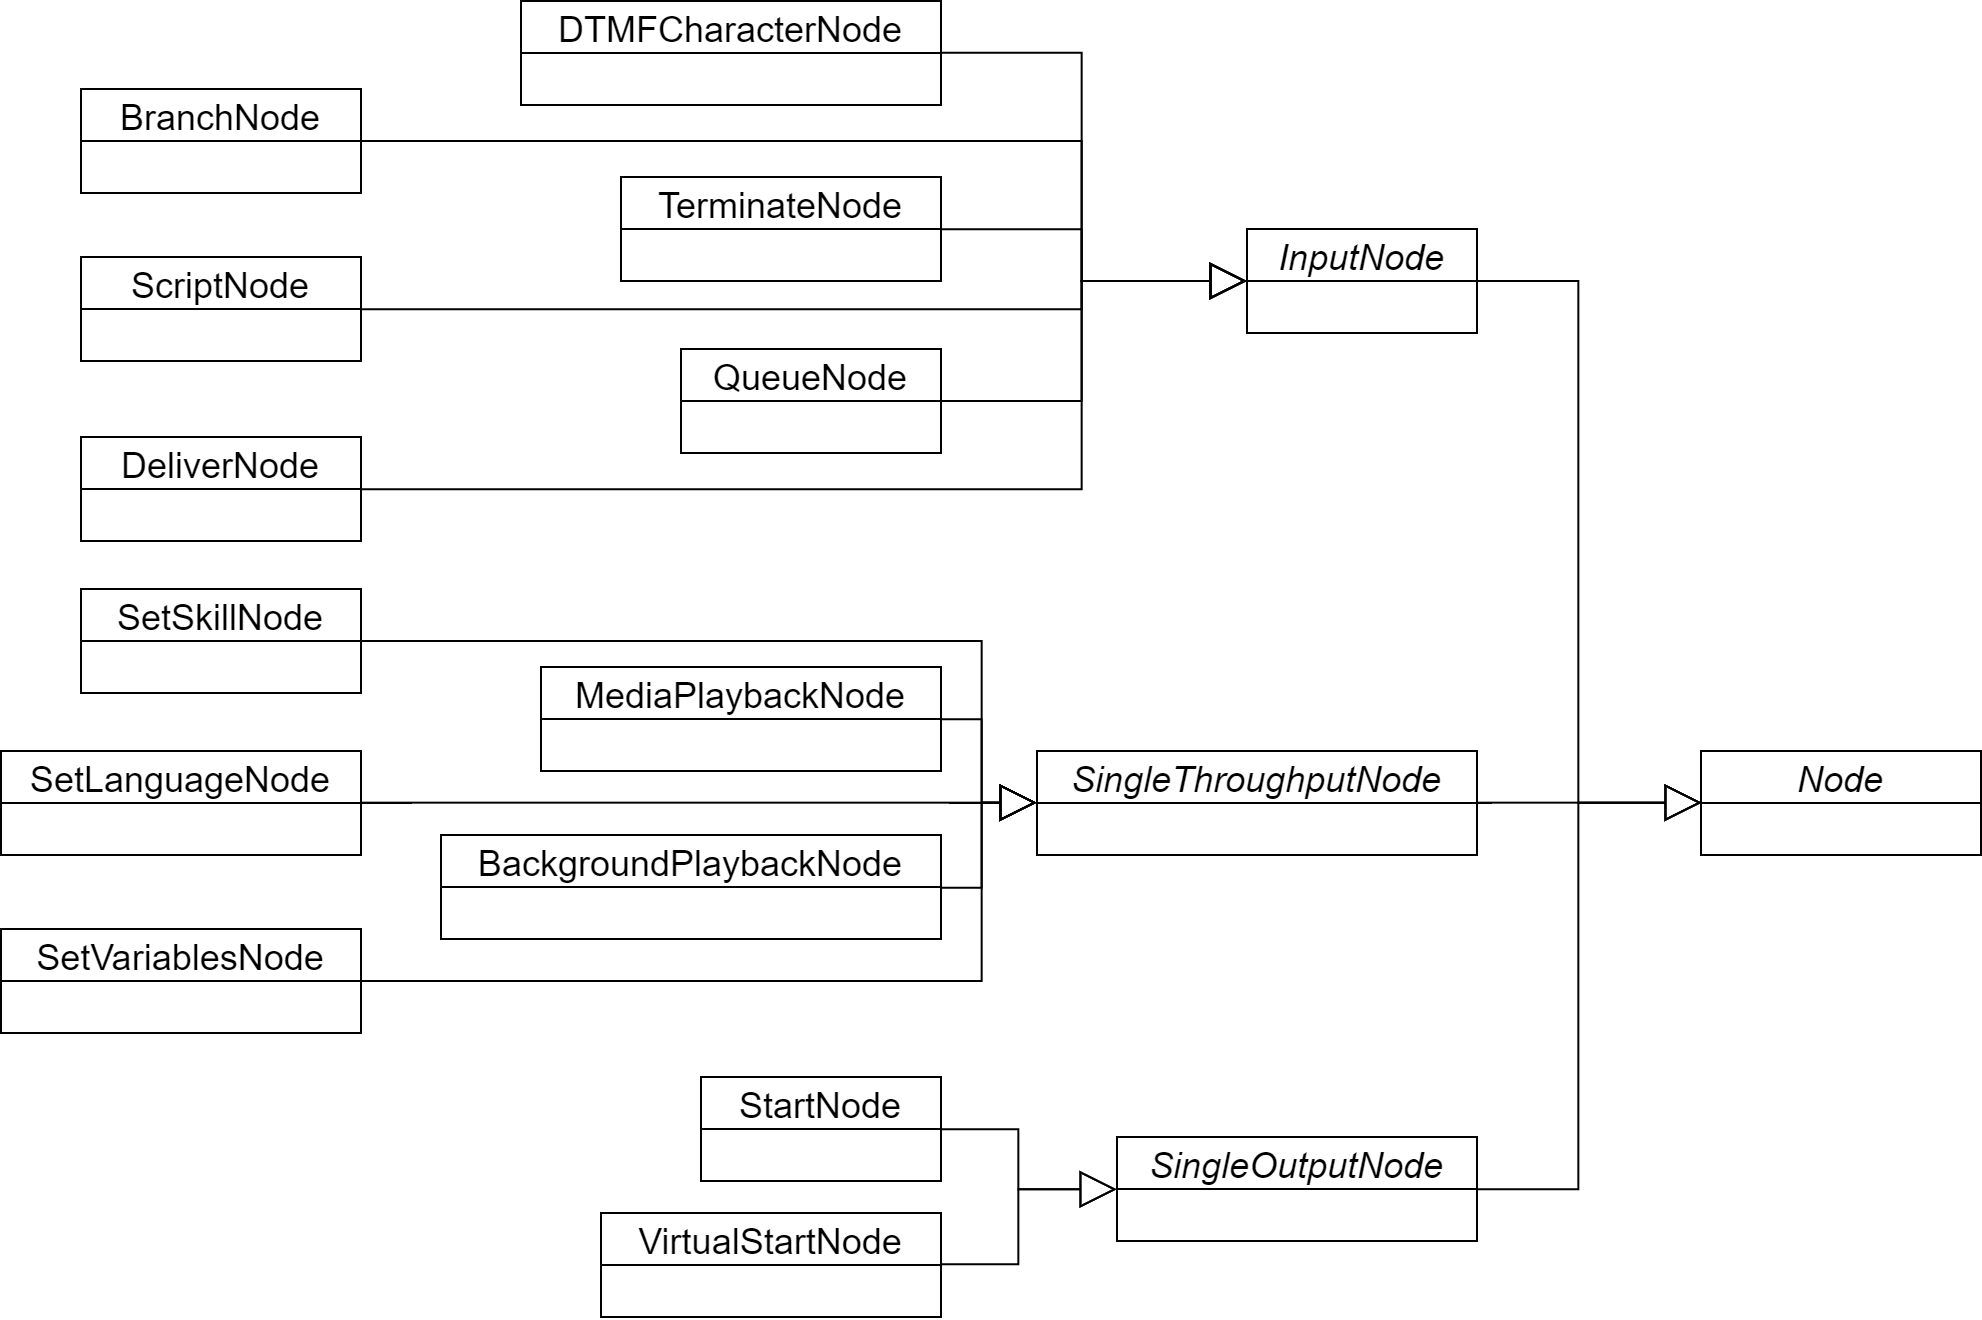
\includegraphics[width=\textwidth]{img/NodeHierarchy.png}
	\caption[Klassenhierarchie der Klasse \texttt{Node}]{\textit{Abgebildet ist die Klasse \texttt{Node} und ihre Subtypen. Jede Instruktion der DSL ist durch einen Subtyp von \texttt{Node} abgebildet. Ob die Klasse als Zwischenstufe von \texttt{InputNode}, \texttt{SingleThroughputNode} oder \texttt{SingleOutputNode} erbt, ergibt sich aus der Anzahl an Ein- und Ausgängen der Instruktion.}}
	\label{fig:UML:Node-Hierarchy}
\end{figure}
\noindent Pro Ausgang einer Instruktion fügt der Konstruktor des entsprechenden \texttt{Node}-Subtyps der Referenzliste der Basisklasse eine neue Referenz vom Typen \texttt{Output} hinzu. Im Konstruktor wird ebenfalls \texttt{Input} initialisiert: Hat die Instruktion einen Eingang, wird die \texttt{Input}-Referenz instanziert, andernfalls bleibt sie null. Viele Instruktionen haben die gleiche Anzahl an Ausgängen und einen Eingang. Daher existieren zusätzliche Subtypen, welche die Initialisierungsarbeit übernehmen: \texttt{Inputnode} für Instruktionen, die einen Eingang haben, \texttt{SingleOutputNode} für Instruktionen, die einen einzelnen Ausgang haben und \texttt{SingleThroughputNode} für Instruktionen, die einen Ein- und einen einzelnen Ausgang haben. Alle dreizehn Subtypen für die Instruktionen erben von diesen drei Klassen und passen dort wo nötig ihre \texttt{Input}- und \texttt{Output}-Konfiguration an. Beispielsweise erbt \texttt{DTMFCharacterNode} von \texttt{InputNode} und fügt der eigenen \texttt{Output}-Referenzliste dreizehn neue \texttt{Output}-Instanzen hinzu.
\newline
Die Klasse \texttt{Input} ist simpel: Sie zeigt über eine Referenz vom Typen \texttt{Node} auf ihre besitzende Instruktion. Die Klasse \texttt{Output} hingegen besitzt mehrere Daten. Sie speichert den Bezeichner des Ausgangs als String, einen weiteren String namens \texttt{DisplayString}, welcher vom Benutzer editiert werden kann und auf der Benutzeroberfläche angezeigt wird, einen Boolean namens \texttt{Visible}, welcher bestimmt ob der Ausgang im Diagramm des Konversationsroutings angezeigt wird, und eine Referenz vom Typ \texttt{Input} auf einen Eingang, falls der Ausgang mit einem solchen verbunden sein sollte. Durch letztere \texttt{Input}-Referenz sind die Verbindungen im Konversationsrouting zwischen den Instruktionen implizit gegeben. Zusätzlich existiert eine weitere Klasse namens \texttt{Connector}, welche eine Verbindung explizit definiert. Sie besitzt Referenzen auf diejenigen \texttt{Input}- und die \texttt{Output}-Instanzen, welche in einem Konversationrouting verbunden sind.
\newline
Benutzerdefinierte Variablen und Funktionen sind über die eigenen Klassen \texttt{Va\-ri\-a\-ble} und \texttt{Function} abgebildet. \texttt{Variable} besitzt einen Namen vom Typ String und einen Typ, der über einen Enum namens \texttt{VariableType} modelliert ist. Dieser Enum beinhaltet die in \ref{subsec:Variablen} aufgezählten Typen. \texttt{Function} speichert ebenfalls einen Namen vom Typ String und einen Rückgabetyp, welcher über einen Enum mit Namen \texttt{FunctionReturnType} abgebildet ist. Zusätzlich wird der Funktionskörper mit Namen \texttt{Body} als String gespeichert. Die Parameter einer Funktion werden über eine Liste von Referenzen auf Instanzen der Klasse \texttt{Parameter} modelliert. \texttt{Parameter} besitzt, ähnlich wie die Klasse \texttt{Variable}, einen Namen als String und einen Typ als \texttt{VariableType}. Die Klasse \texttt{Flow} vereint alle oben genannten Klassen: Sie beinhaltet Listen mit Referenzen auf alle \text{Node}-, \texttt{Connector}-, \texttt{Function}- und \texttt{Variable}-Instanzen eines Konversationsroutings. 



\subsection[Die ViewModel-Schicht]{Die ViewModel-Schicht: FlowDiagramViewModel, CodeEditorViewModel, FunctionCollectionEditorViewModel}
\label{subsec:Die Viewmodel-Schicht}
In der ViewModel-Schicht werden die Klasseninstanzen der Model-Schicht so aufbereitet, dass die View-Schicht sie per Datenbindung repräsentieren kann. Die ViewModel-Schicht reagiert auch auf Eingaben des Benutzers und manipuliert das zu Grunde liegende Model nach dessen Wünschen. Der wichtigste Teil der ViewModel-Schicht ist in Abbildung \ref{fig:UML:FlowViewModel} dargestellt.
\begin{figure} %[hbtp]
	\centering
		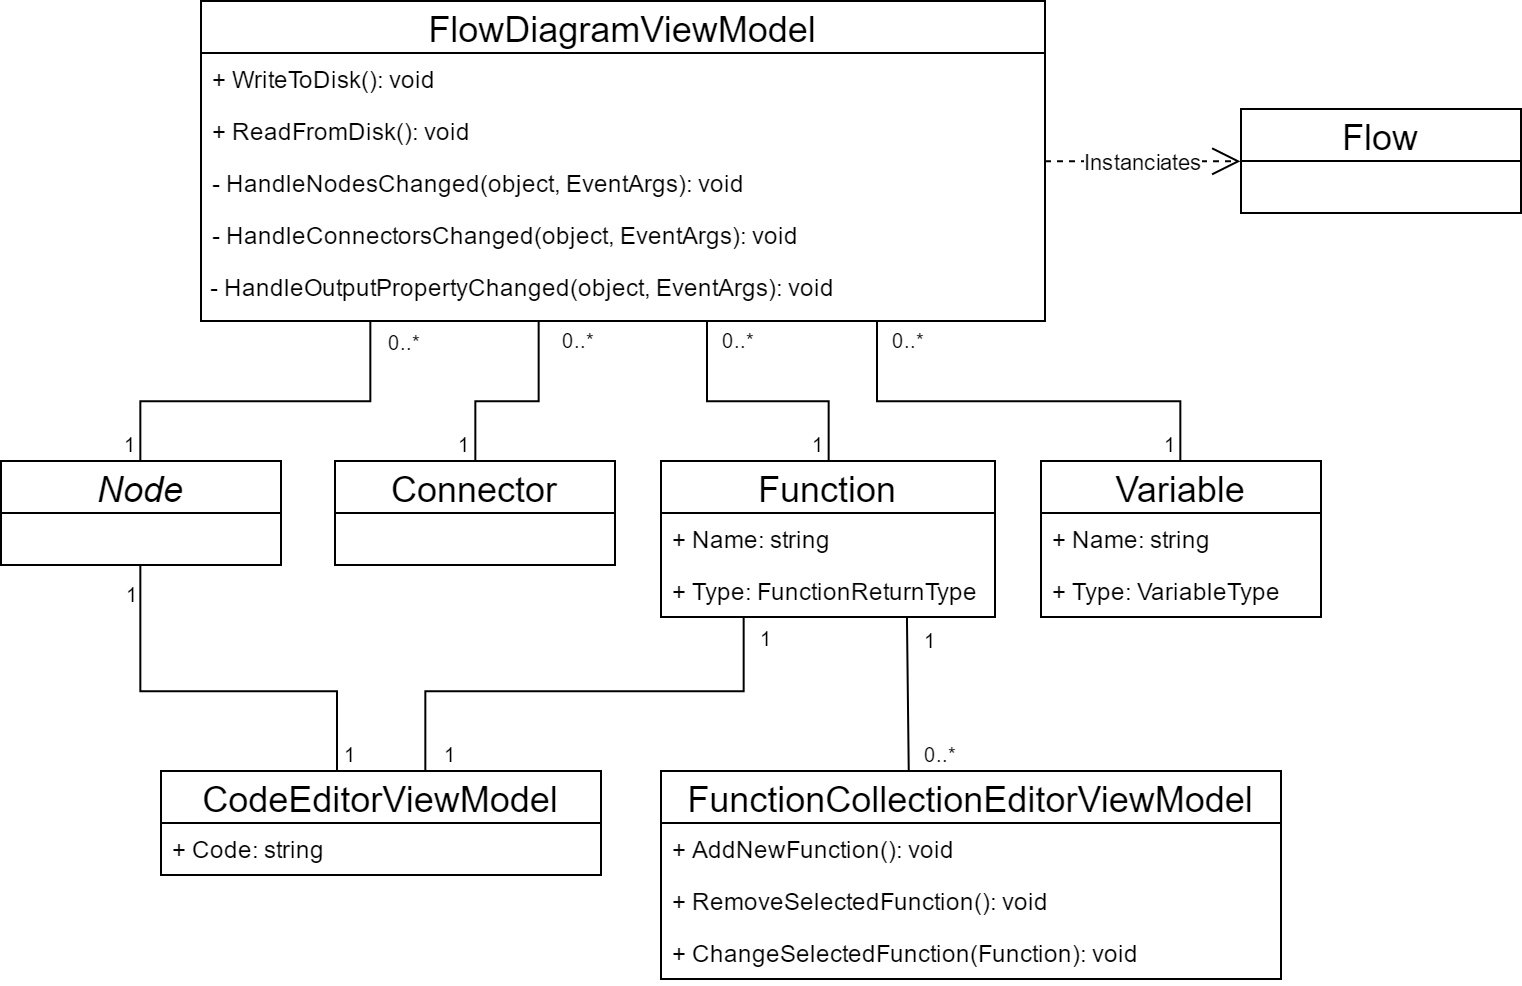
\includegraphics[width=\textwidth]{img/FlowDiagramViewModelUML.png}
	\caption[Klassenstruktur der ViewModel-Schicht]{\textit{Zu sehen sind die beiden ViewModel \texttt{FlowDiagramViewModel} und \texttt{CodeEditorViewModel}. Ersteres verwaltet Listen mit \texttt{Node}-, \texttt{Con\-nec\-tor}-, \texttt{Variable}- und \texttt{Function}-Instanzen, die beim Instanzieren der Klasse \texttt{Flow} benötigt werden. Letzteres übernimmt die Präsentationslogik für den Code-Editor, indem es Referenzen auf die zu bearbeitenden \texttt{Node}- und \texttt{Function}-Instanzen verwaltet und den Code in Form eines Strings für die Datenbindung bereit stellt.}}
	\label{fig:UML:FlowViewModel}
\end{figure}
Der Hauptbestandteil der Schicht ist die Klasse \texttt{FlowDiagramViewModel}. Diese besitzt als Membervariablen Listen auf Referenzen der Model-Komponenten \texttt{Node}, \texttt{Connector}, \texttt{Variable} und \texttt{Function}. Diese Listen sind vom .NET-Listen-Typ \texttt{ObservableCollection}, welcher ein Event auslöst, falls Objekte hinzugefügt oder entfernt werden und sind per Devexpress-Datenbindung an die View-Schicht gekoppelt. Das heißt, wenn auf der View-Schicht Elemente des Modells wie zum Beispiel neue \texttt{Node}- oder \texttt{Connector}-Objekte hinzugefügt werden, aktualisieren sich die entsprechenden Listen im \texttt{FlowDiagramViewModel}. Zusätzlich werden dadurch Events ausgelöst, auf die \texttt{FlowDiagramViewModel} in den Methoden \texttt{HandleNodesChanged} und \texttt{HandleConnectorsChanged} reagiert. Dies wird dazu genutzt, die Referenzen zwischen den Klassen \texttt{Input} und \texttt{Output} aktuell zu halten: Wird ein \texttt{Connector} der Liste hinzugefügt, löst das ein Event aus. Auf dieses Event wird reagiert, indem die Input-Membervariable der im \texttt{Connector} referenzierten \texttt{Output}-Instanz gesetzt wird. 
\newpage
\noindent Diese wird auf die \texttt{Input}-Instanz gesetzt, die ebenfalls im neuen \texttt{Connector} verlinkt ist. Der Vorgang wird rückgängig gemacht, wenn ein \texttt{Connector} entfernt wird. Die Datenbindung funktioniert auch umgekehrt: Wenn sich die Input-Referenz eines Outputs ändert, wird ein Event ausgelöst, welches in der Methode \texttt{HandleOutputPropertyChanged} behandelt wird. Dort wird ein neuer Connector mit entsprechenden \texttt{Input}- und \texttt{Output}-Referenzen hinzugefügt. Der grundsätzliche Ablauf der Kommunikation zwischen ViewModel und View ist in Abb. \ref{fig:UML:MVVMSequence} verbildlicht.
\begin{figure} %[hbtp]
	\centering
		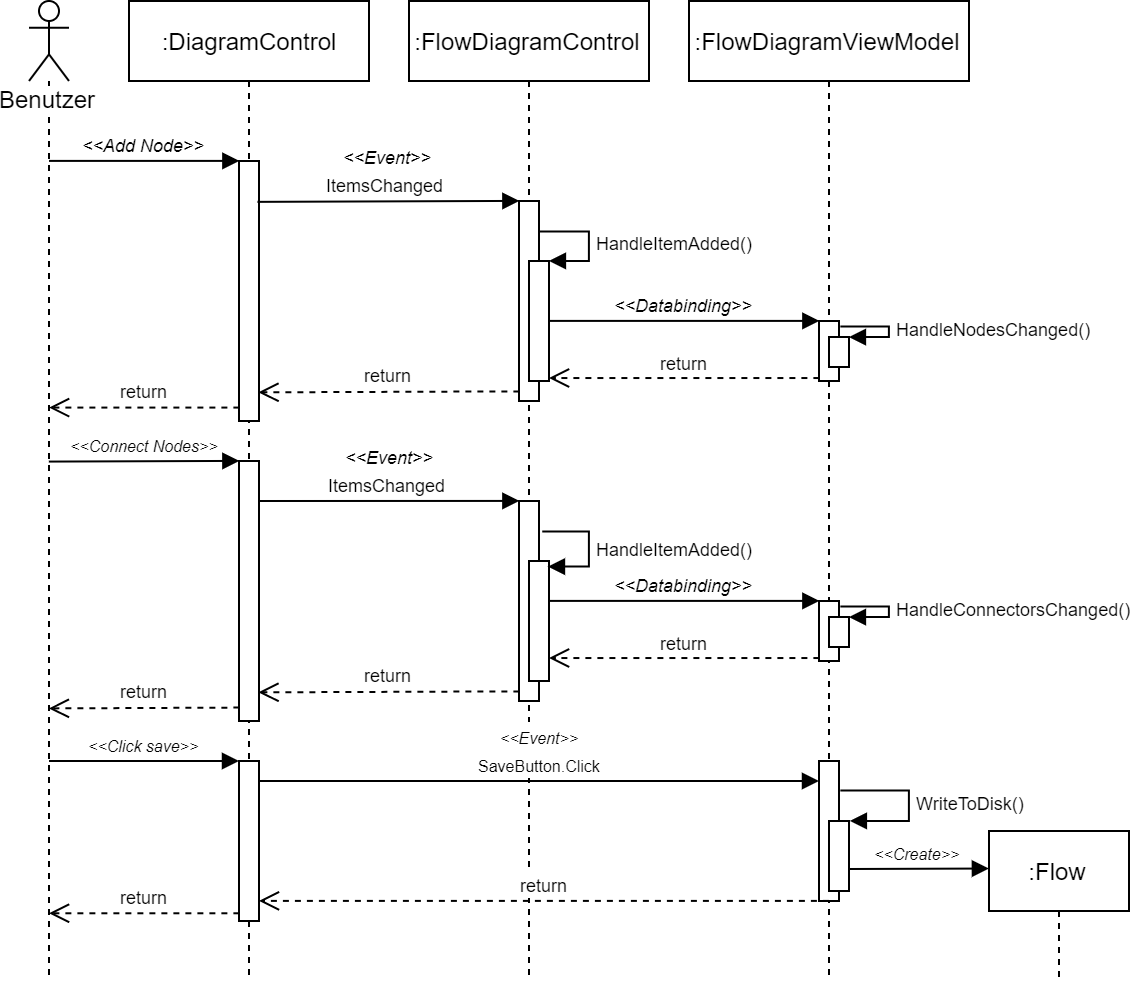
\includegraphics[width=\textwidth]{img/MVVMSequence.png}
	\caption[Kommunikationsablauf zwischen View- und ViewModel-Schicht]{\textit{Der Ablauf der Kommunikation zwischen der View- und der ViewModel-Schicht. Interagiert der Benutzer mit dem View, zum Beispiel durch das Hinzufügen von \texttt{Node}- oder \texttt{Connector}-Instanzen, werden entsprechende Events ausgelöst. Auf diese reagiert die abgeleitete View-Klasse \texttt{FlowDiagramControl} und aktualisiert ihre Daten mit den neuen Objekten. Das ViewModel erhält die aktualisierten Daten über die Datenbindung des Frameworks und kann so, wenn der Benutzer das Konversationsrouting speichern möchte, die Klasse \texttt{Flow} der Model-Schicht instanzieren.}}
	\label{fig:UML:MVVMSequence}
\end{figure}
\texttt{FlowDiagramViewModel} übernimmt mittels der beiden Kommandos \texttt{Write\-To\-Disk} und \texttt{Read\-From\-Disk} auch das Speichern und Laden von Konversationsroutings. Dafür wird mit den Listen der \texttt{Node}-, \texttt{Connector}-, \texttt{Variable}- und \texttt{Function}-Instanzen ein \texttt{Flow}-Objekt instanziert und serialisiert. Pfade für die zu schreibenden beziehungsweise lesenden Dateien werden über Dialoge vom Benutzer abgefragt.
\newline
Einige Instruktionen eines Konversationsroutings benötigen die Möglichkeit, Code einzugeben. Zu diesem Zweck existiert ein weiteres ViewModel, welches dem eingebauten Code-Editor zu Grunde liegt. \texttt{CodeEditorViewModel} beinhaltet einen String, welcher den Code enthält. Dieser ist per Datenbindung an den Text des Code-Editors gebunden. Zusätzlich enthält \texttt{CodeEditorViewModel} entweder eine Referenz auf die zu bearbeitende \texttt{SkriptNode}-, \texttt{BranchNode}- oder \texttt{Function}-Instanz. Eine Aufgabe von \texttt{CodeEditorViewModel} ist es, den im Editor eingegebenen Code synchron mit dem Code in der jeweiligen \texttt{Node} oder \texttt{Function} zu halten. 
\newline
Damit der Benutzer die selbst definierten Funktionen verwalten kann, existiert zusätzlich ein Funktions-Editor, in dem neue Funktionen angelegt, gelöscht oder bearbeitet werden können. Für diesen Editor wird ein eigenes ViewModel namens \texttt{FunctionCollectionViewModel} verwendet. Es beinhaltet eine Referenz auf die Liste der Funktionen, die sich im \texttt{FlowDiagramViewModel} befinden und wendet das Ändern, Löschen oder Hinzufügen von Funktionen auf diese Liste an.

\subsection[Die View-Schicht]{Die View-Schicht: FlowDiagramView, FlowDiagramControl, FlowDiagramItem}
Die View-Schicht übernimmt alle Elemente der grafischen Benutzeroberfläche, die der Benutzer unmittelbar sieht und mit denen er interagiert. Das Hauptelement der View-Schicht ist die Klasse \texttt{FlowDiagramView}, welche von der Framework-Klasse \texttt{UserControl} erbt. \texttt{FlowDiagramView} umfasst alle Windows Forms-Controls, die zum Darstellen des Editors benötigt werden und übernimmt zusätzlich die Konfiguration des MVVM-Frameworks während der Initialisierungsphase der Be\-nutz\-er\-ober\-fläche.
\newline  
Das wichtigste Element der Benutzeroberfläche ist das Control \texttt{Flow\-Dia\-gram\-Con\-trol}, welches  die konkrete Syntax des Konversationsroutings darstellt. In Abbildung \ref{fig:UML:FlowView} ist schematisch dargestellt, wie es in die Klassenstruktur der View-Schicht eingefügt ist. 

\begin{figure} %[hbtp]
	\centering
		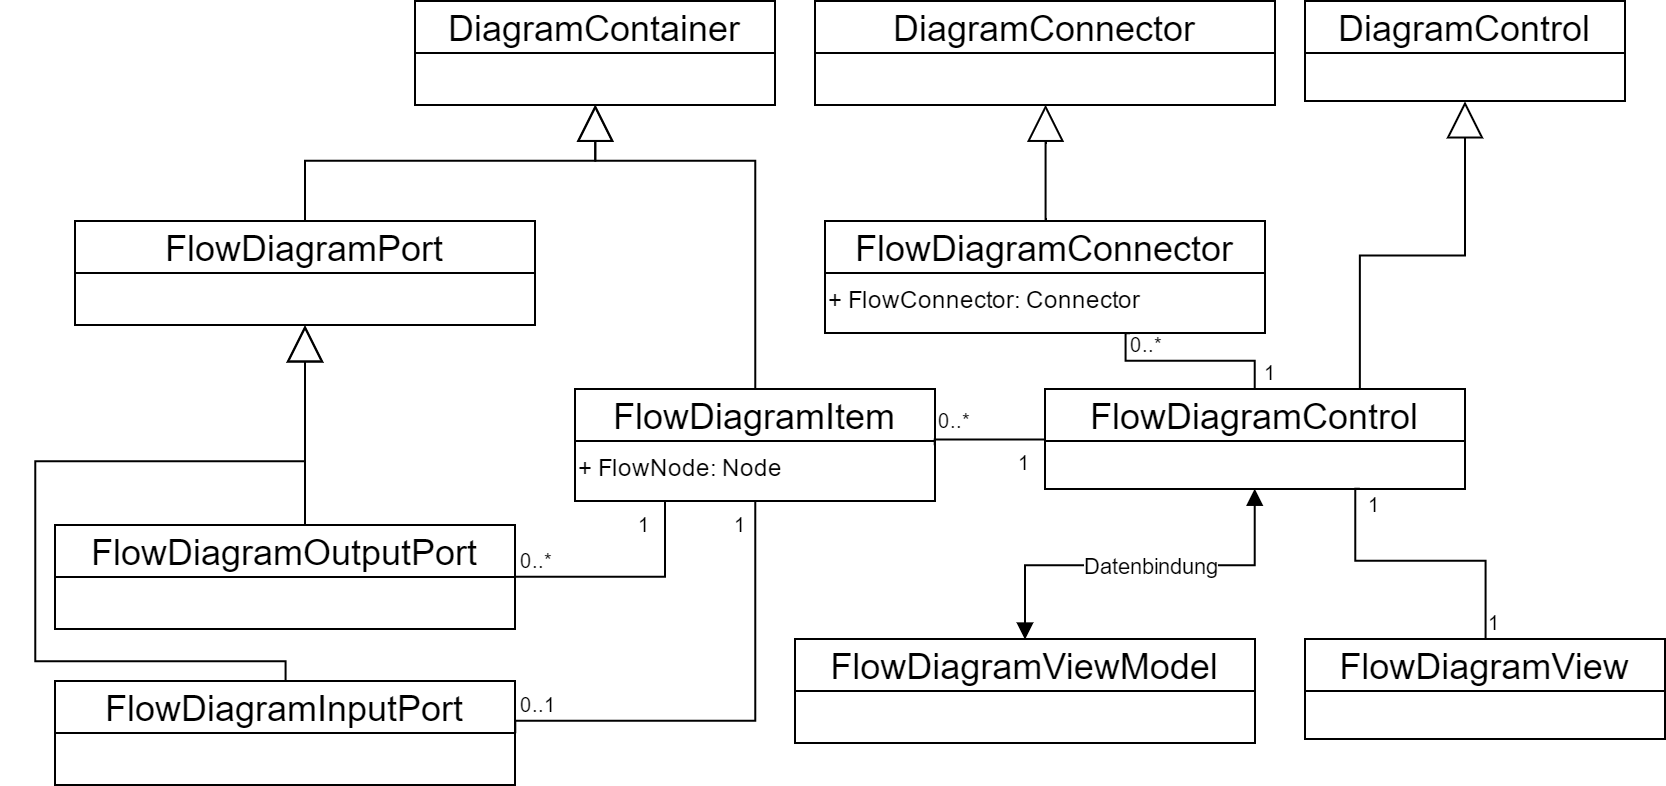
\includegraphics[width=\textwidth]{img/FlowViewUML.png}
	\caption[Klassenstruktur der View-Schicht]{\textit{Abgebildet ist ein Teil der View-Schicht. Zu sehen ist \texttt{FlowDiagramView}, welche über eine Instanz von \texttt{FlowDiagramControl} verfügt. \texttt{FlowDiagramControl} beinhaltet die Klassen \texttt{FlowDiagramItem} und \texttt{FlowDiagramConnector}, welche die \texttt{Node}- und \texttt{Connector}-Instanzen der Model-Schicht visualisieren. Über das ViewModel erhält \texttt{FlowDiagramControl} per Datenbindung Zugriff die zu visualisierenden Daten.}}
	\label{fig:UML:FlowView}
\end{figure}
\noindent Es basiert auf der Devexpress-Klasse \texttt{DiagramControl}, die es Benutzern ermöglicht, Diagramme mit geometrischen Formen und Verbindungen zu gestalten. \texttt{Flow\-Dia\-gram\-Con\-trol} ist von dieser Klasse abgeleitet und erweitert sie um die Fähigkeit, ein Modell der DSL per Datenbindung darzustellen. Dafür sind in \texttt{FlowDiagramControl} Listen vom Typ \texttt{ObservableCollection} als Membervariablen angelegt, welche die Elemente des aktuellen DSL-Modells enthalten. Diese Listen existieren analog zur Klasse \texttt{FlowDiagramViewModel} aus Abschnitt \ref{subsec:Die ViewModel-Schicht}. Durch die Datenbindung zwischen \texttt{FlowDiagramControl} und \texttt{FlowDiagramViewModel} werden die Inhalte aller Listen synchron gehalten. Die Aufgabe von \texttt{FlowDiagramControl} ist es, auf Interaktionen des Benutzers so zu reagieren, dass die Listen entsprechend aktualisiert werden. Zu diesem Zweck ist diese Klasse in einigen Aspekten gegenüber \texttt{DiagramControl} wie folgt angepasst und spezialisiert. Für ein Devexpress-\texttt{DiagramControl} kann eine Auswahl von sogenannten Stencils, also für das Diagramm verfügbare Formen, dem Control hinzugefügt werden. Jedes Stencil verfügt über ein Objekt der Klasse \texttt{FactoryItemTool}, welches eine Instanz vom Interface-Typ \texttt{IDiagramItem} erzeugt. Wird ein Stencil aus der Toolbox in das Diagramm per Drag and Drop eingefügt, erzeugt das zugehörige \texttt{FactoryItemTool} ein entsprechendes Objekt, welches \texttt{IDiagramItem} implementiert. \texttt{IDiagramItem} stellt Methoden zu Verfügung, die \texttt{DiagramControl} benötigt um Objekte grafisch darzustellen. \texttt{FlowDiagramControl} ist so konfiguriert, dass jeder \texttt{Node}-Subtyp, also jede Instruktion der DSL, als eigenes Stencil dem Control hinzugefügt ist. Die Instanzen von \texttt{FactoryItemTool} für jedes dieser Stencil erzeugen ein Objekt vom Typ \texttt{FlowDiagramItem}. \texttt{Flow\-Dia\-gram\-Item} ist die visuelle Repräsentation einer Konversationsrouting-Instruktion und erbt von der Devexpress-Klasse \texttt{DiagramContainer}, welche \texttt{IDiagramItem} implementiert. \texttt{Flow\-Dia\-gram\-Item} besitzt eine Referenz auf ein Objekt vom Typ \texttt{Node}. Im Konstruktor von \texttt{FlowDiagramItem} wird das visuelle Erscheinungsbild einer einzelnen Instruktion initialisiert: Dabei werden Klassen vom Devexpress-Typ \texttt{DiagramShape} zu einer Liste hinzugefügt, welche dann vom Framework gezeichnet werden und verschiedene geometrische Formen annehmen können. \texttt{Flow\-Dia\-gram\-Item} fügt der Liste von \texttt{DiagramShape}-Instanzen ein blaues Rechteck für den Körper, ein weißes Rechteck für die Instruktionsüberschrift sowie kleinere rote und grüne Rechtecke für Instruktionsaus- und Eingänge hinzu. Die Rechtecke für Ein- und Ausgänge werden durch die eigens implementierten Klassen \texttt{FlowDiagramInputPort} und \texttt{FlowDiagramOutputPort} repräsentiert. Beide Klassen erben von der gemeinsamen Basis-Klasse \texttt{Flow\-Dia\-gram\-Port}, welche wiederum \texttt{DiagramContainer} erweitert. Diese Port-Klassen bestimmen das visuelle Erscheinungsbild der zu zeichnenden Rechtecke und ermöglichen es \texttt{FlowDiagramItem} Ausgänge zu beschriften oder aus- und einzublenden. Wie viele Aus- und Eingänge die jeweilige zu visualisierende Instruktion besitzt, wird aus dem Subtyp der \texttt{Node}-Referenz ermittelt, die in \texttt{FlowDiagramItem} hinterlegt ist.
\newline
Wird nun vom Benutzer ein Stencil aus der Toolbox ausgewählt und in das Modellierungsfenster gezogen, erzeugt die zugehörige Instanz von \texttt{FactoryItemTool} ein \texttt{FlowDiagramItem}. Dieses \texttt{FlowDiagramItem} wird mit einer Referenz auf eine neu erstellte Instanz des \texttt{Node}-Subtyps der ausgewählten Instruktion initialisiert. \texttt{DiagramControl} löst dann ein Event aus, das signalisiert, dass sich die Liste an Diagramm-Elementen verändert hat. \texttt{FlowDiagramControl} reagiert auf dieses Event seiner Basisklasse, indem es die \texttt{Node}-Referenz aus dem hinzugefügten \texttt{FlowDiagramItem} zu der Liste der \texttt{Node}-Instanzen hinzufügt, die per Datenbindung an das \texttt{FlowDiagramViewModel} gebunden sind. Umgekehrt reagiert \texttt{FlowDiagramControl} auch auf Events, die ausgelöst werden, wenn die Liste der \texttt{Node}-Instanzen durch \texttt{FlowDiagramViewModel} verändert wird. In diesem Fall wird ein neues \texttt{FlowDiagramItem} mit einer Referenz auf die hinzugefügte \texttt{Node}-Instanz erzeugt, sodass diese \texttt{Node}-Instanz auf der Benutzeroberfläche zu sehen ist. Analog verhält sich das System wenn \texttt{Node}-Instanzen oder \texttt{FlowDiagramItem}-Instanzen gelöscht werden, nur dass in diesem Fall Elemente entfernt werden.
\newline
Um die Verbindungen zwischen Instruktionen zu modellieren, wird ähnlich vorgegangen. \texttt{FlowDiagramControl} überschreibt die geerbte Methode \texttt{CreateConnector}, welche vom Framework aufgerufen wird, wenn der Benutzer eine Verbindung zwischen Diagrammelementen zieht. Die Methode liefert eine Instanz von \texttt{Flow\-Dia\-gram\-Con\-nec\-tor} zurück, in der eine Referenz auf einen \texttt{Connector} der Model-Schicht hinterlegt ist. Wird ein \texttt{FlowDiagramConnector} dem Diagramm hinzugefügt, wird über ein entsprechendes Event eine neue \texttt{Connector}-Instanz der per Datenbindung synchronisierten Liste hinzugefügt. In \texttt{FlowDiagramViewModel} wird dementsprechend ebenfalls eine neue \texttt{Connector}-Instanz hinzugefügt und die \texttt{Input}- und \texttt{Output}-Referenzen der im \texttt{Connector} betroffenen Ein- und Ausgänge werden aktualisiert. Wird eine \texttt{Connector}-Instanz der Modelschicht hinzugefügt, läuft der Prozess rückwärts ab. Das heißt, über die synchronisierte Liste der \texttt{Connector}-Instanzen wird ebenfalls in \texttt{FlowDiagramControl} ein Event ausgelöst, sodass das Control dem Diagramm einen neuen \texttt{Flow\-Dia\-gram\-Co\-nnec\-tor} hinzufügen kann. Beim Entfernen von \texttt{Connector}-Instanzen wird der Prozess gleich behandelt, nur dass Referenzen entsprechend entfernt werden.      

\section{Transformation}
\label{sec:Transformation}

\subsection{Konzept}
\label{subsec:Konzept}
Die Transformation ist der Schritt in der Verarbeitungskette, in der aus einem semantischen Modell, welches in der Form eines Objekt-Graphen aus Abschnitt \ref{subsec:Die Model-Schicht} vorliegt, die CIL-Syntax generiert wird. Diese kann anschließend kompiliert und ausgeführt werden. Ein DSL-Modell wird auf eine zu generierende Klasse abgebildet, welche das gewünschte Verhalten des Modells implementiert. Diese Klasse erbt von einer abstrakten Basisklasse mit dem Namen \texttt{ACDCallRoutingBehaviorBase}, welche die abstrakte Methoden \texttt{StartAsync} und \texttt{VirtualStartAsync} zur Verfügung stellt. Die vom Transformationsalgorithmus generierte Klasse implementiert \texttt{Start\-Async} und \texttt{VirtualStartAsync} so, dass beim Aufruf das vom Benutzer jeweils spezifizierte Konversationsrouting ausgeführt wird.
\newline 
Die Instruktionen des Konversationsroutings werden als Membermethoden der Klasse abgebildet. In der generierten Klasse existiert für jede Instruktion eine eigene Methode, deren Syntax das gewünschte Verhalten der Instruktion umsetzt. Der Bezeichner der Methode trägt den Namen der Instruktion, gefolgt von einer eindeutigen Identifikationsnummer, sodass mehrere Instruktionen des gleichen Typs bei der Generierung der zugehörigen Membermethoden nicht kollidieren. Manche Instruktionen müssen mit der zu behandelnden Konversation interagieren. Zu diesem Zweck steht der generierten Klasse eine API zur Verfügung. Der Zugang zu  dieser API ist eine Membervariable der Klasse \texttt{RoutedAcdCall}, welche in der Basisklasse \texttt{ACDCallRoutingBehaviorBase} angelegt ist und ein Interface namens \texttt{IRoutedAcdCall} implementiert. Soll beispielsweise im Zuge einer Media Playback-Instruktion eine Audio-Datei abgespielt werden, kann Syntax generiert werden, welche die Methode \texttt{PlayAudioAsync} des Interfaces \texttt{IRoutedAcdCall} auf dieser Membervariable aufruft. 
\newline
Die Reihenfolge von Instruktionen in einem Konversationsrouting wird realisiert, indem generierte Methoden die Methoden ihrer Nachfolgeinstruktionen aufrufen. Angenommen, eine Branch-Instruktion hat zwei Ausgänge: Der ''True``-Ausgang zeigt auf eine Media Playback-Instruktion während der ''False``-Ausgang auf die Terminate-Instruktion verweist. Aus diesen drei Instruktionen wird Syntax für drei Membermethoden generiert: Die Methode der Branch-Anweisung wertet den per Parameter übergebenen booleschen Ausdruck aus und ruft im True-Fall die Methode der Media Playback-Instruktion auf. Andernfalls wird die Methode der Terminate-Instruktion aufgerufen. 
\newline
Da es sich bei dem semantischen Modell um einen Graphen und keinen Baum handelt, kann es in Modellen zu Zyklen kommen. Solche potentiell endlosen Konversationsroutings stellen ein Problem dar, denn sie führen zu einer endlosen Rekursion von Methodenaufrufen innerhalb der generierten Klasse und damit zu einem Überlauf des Aufrufstapels. Das Problem wird gelöst, indem eine Instruktion, die eine solche Rekursion startet, die nächste Instruktion in einem .NET-Task auf einem neuen Thread aufruft. Der aktuelle Thread terminiert an der Stelle, an der der neue gestartet wird und ein neuer Aufrufstapel wird angelegt.
\newline
Ein Modell kann vom Benutzer geschriebenen C\#-Code enthalten. Dieser muss in die generierte Klasse integriert werden, um ausführbar zu sein. Benutzerdefinierten Code jedoch einfach in die Syntax für Membermethoden einzufügen birgt Risiken. So hätte der Benutzer in seinem selbstgeschriebenen Code Zugriff auf alle Elemente der generierten Klasse, was zu Problemen führen kann, wenn er Methoden aufruft, die der generierten Klasse vorbehalten sind. Stattdessen wird Code des Benutzers in einer verschachtelten privaten Klasse gekapselt. Die geschachtelte Klasse trägt den Bezeichner ``UserCode'' und kapselt den benutzerdefinierten Code in eigenen Membermethoden. Die umfassende Klasse verfügt als Membervariable über eine Instanz der Klasse \texttt{UserCode} und kann so den Code des Benutzers ausführen.  Enthält eine Instruktion Benutzer-Code, wird sie also auf zwei verschiedene Methoden abgebildet: Eine Membermethode der Klasse \texttt{UserCode}, und eine Membermethode der umfassenden Klasse. Die Membermethode der umfassenden Klasse ruft die zweite in \texttt{UserCode} enthaltene Methode auf, um den Benutzercode auszuführen. Ist beispielsweise eine Branch-Instruktion im Konversationsrouting integriert, wird der dort enthaltene boolesche Ausdruck in einer eigenen Membermethode in der Klasse \texttt{UserCode} angelegt. Die Branch-Instruktion wird zusätzlich als Membermethode der umfassenden Klasse abgebildet, welche dann die zugehörige Methode in \texttt{UserCode} aufruft. Da boolesche Ausdrücke einen Boolean zurückliefern, gibt auch die in UserCode angelegte Membermethode einen Boolean zurück, welcher dann in der aufrufenden Methode dazu verwendet wird, um zu entscheiden, welcher Ausgang der Instruktion benutzt werden soll.
\newline
Vom Benutzer definierte Variablen und Funktionen sind in allen Instruktionen verwendbar, in denen der Benutzer eigenen Code angeben kann. Da Code des Benutzers in der Klasse \texttt{UserCode} abgebildet wird, werden auch die vom Benutzer angelegten Variablen und Funktionen in dieser Klasse jeweils als private Membervariablen und -funktionen angelegt. Die vordefinierten Variablen \texttt{Skill} und \texttt{Language} sind ebenfalls über die Klasse \texttt{UserCode} verfügbar: Sie sind als Properties vom Typ String in \texttt{UserCode} umgesetzt. Die Getter und Setter dieser String-Properties werden mit einer Instanz der Klasse \texttt{PredefinedVariables} umgesetzt, welche ein Interface namens \texttt{IPredefinedVariables} implementiert. \texttt{PredefinedVariables} hat die Aufgabe, die Strings, mit denen der Benutzer in seinem eigenen Code arbeitet, auf Datenstrukturen abzubilden, die die ausführende Routing Engine verwendet. Wird beispielsweise der Setter der \texttt{Language}-Variable mit einem als String übergebenen Namen aufgerufen, überprüft \texttt{PredefinedVariables}, ob in der Routing Engine eine Sprache mit diesem Namen existiert und weist der Konversation diese Sprache zu. 
\newline
Einige Aufrufe der API zur Interaktion mit dem eingehenden Ruf müssen den Programmfluss des Konversationsroutings zeitweise anhalten. So muss beispielsweise bei der Ausführung einer Media Playback-Instruktion darauf gewartet werden bis die Audiodatei zu Ende ist, bevor die nächste Instruktion ausgeführt werden kann. Der ausführende Thread der Routing Engine blockiert während dieser Warte-Zeit jedoch nicht, um die Performanz der Routing Engine nicht unnötig zu beeinträchtigen. Umgesetzt wird dies mit .NETs System der asynchronen Methodenausführung, welches das Blockieren von Threads umgeht (siehe \ref{subsec:Asynchrone Methodenausfuehrung}). Dazu werden Instruktionen, welche asynchrone API-Methoden aufrufen, selber auf asynchrone Methoden abgebildet. Entsprechend werden asynchrone Methoden, welche Instruktionen abbilden, mit dem \texttt{await}-Operator aufgerufen.

\subsection{Beispiel}
\label{subsec:Beispiel}
Folgendes Beispiel soll die Transformation eines Konversationsroutings zu CIL-Syntax besser veranschaulichen. In Abb. \ref{fig:FlowToCode} ist ein einfaches Konversationsrouting dargestellt. 

\newpage

\begin{figure} %[hbtp]
	\centering
		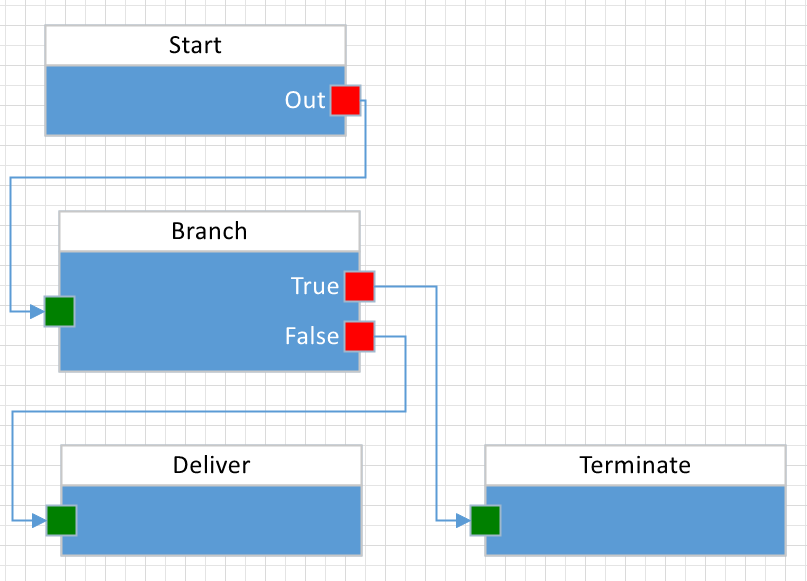
\includegraphics[width=0.7\textwidth]{img/FlowToCodeExample.png}
	\caption[Beispielhaftes Konversationsrouting zur Veranschaulichung der Transformation zu CIL-Syntax]{\textit{Beispielhaftes Konversationsrouting zur Veranschaulichung der Transformation zu CIL-Syntax.}}
	\label{fig:FlowToCode}
\end{figure}
\noindent Die CIL-Syntax, die aus einem solchen Modell generiert wird, ist im Folgenden dargestellt. Bei diesem Beispiel ist zu beachten, dass bei der Transformation nicht wirklich konkrete C\#-Syntax generiert wird, sondern ihr abstraktes Gegenstück in Form eines Rosyln-\texttt{SyntaxTree}-Objekts. Für die Illustration des Transformationskonzeptes ist die Syntax hier jedoch konkret dargestellt.

\lstinputlisting[breaklines=true, style=sharpc, language=custom]{code/FlowToCode.cs}

\noindent Am Anfang des Listings steht die Deklaration einer öffentlichen Klasse namens \texttt{GeneratedConversationBehavior}, die von \texttt{ACDCallRoutingBehavior} erbt. Dies ist die Klasse, in der die Instruktionen als Membermethoden abgebildet werden. In dieser Klasse wird als nächstes eine private Klasse \texttt{UserCode} definiert. In \texttt{UserCode} sind die vordefinierten Variablen \texttt{Skill} und \texttt{Language} definiert, welche über ihre Getter und Setter auf eine private Instanz von \texttt{PredefinedVariable} zugreifen. Zusätzlich existiert eine Methode mit dem Namen \texttt{BranchNode} gefolgt von einer einzigartigen Kennnummer. Diese Methode enthält den vom Benutzer spezifizierten Ausdruck der für die Branch-Instruktion ausgeführt werden soll. Dementsprechend wird ein boolescher Wert zurückgeliefert. In diesem Beispiel vergleicht die Branch-Instruktion also die aktuelle Sprache, welche in der vordefinierten Variable \texttt{Language} gespeichert ist, mit dem String ``Deutsch''. 
\newline
Nach der Klasse \texttt{UserCode} folgt die eigentliche Implementierung des Konversationsroutings. Im Konstruktor der Klasse \texttt{GeneratedConversationBehavior} werden Abhängigkeiten zum Rest des Systems initialisiert: Mittels einer Implementierung des Interfaces \texttt{IRoutedAcdCall} wird auf eine API zur Beeinflussung des eingehenden Anrufes zugegriffen. Die beiden Instanzen von \texttt{IReadOnlyRepository} stellen Methoden zur Verfügung, um auf die dem System bekannten Sprachen und Wissensbereiche zuzugreifen. Die drei Interface-Instanzen werden an die Basisklasse \texttt{ACDCallRoutingBehaviorBase} weitergeleitet. Im Konstruktor wird außerdem die private Instanz von \texttt{UserCode} initialisiert, welcher eine \texttt{PredefinedVariables}-Instanz aus der Basis-Klasse übergeben wird. Die restlichen Methoden der Klassen stellen die Abbildung der Instruktionen des Konversationsroutings dar. Der Lesbarkeit halber werden die eindeutigen Kennnummern, welche die Bezeichner von Instruktionsmethoden begleiten, im Folgenden ausgelassen. Die Start-Instruktion wird auf die Methode \texttt{StartAsync} abgebildet. Hier wird dem Routing gemäß sofort die Methode der Branch-Instruktion \texttt{BranchNode} aufgerufen, welche zuerst den vom benutzerdefinierten Code aus der Klasse \texttt{UserCode} aufruft, und das Ergebnis dessen als Bedingung in eine If-Abfrage einsetzt. Je nachdem welches Ergebnis zurückgeliefert wird, wird entweder die Methode der Deliver- oder der Terminate-Instruktion aufgerufen. \texttt{TerminateNode} ruft über die Membervariable \texttt{Conversation} der Basisklasse die API-Methode \texttt{TerminateAsync} auf, welche den eingehen Anruf beendet. Ähnlich läuft es in \texttt{DeliverNode} ab: Hier wird der Ruf mittels der API-Methode \texttt{DeliverAsync} der Ruf an einen Agenten zugestellt. Die dabei übergebene SIP-URI ist ein Parameter der Deliver-Instruktion.
\newline
Wird die Klasse \texttt{GeneratedConversationBehavior} nun von der Routing Engine instanziert und in einer Variable vom Typ \texttt{ACDCallRoutingBehaviorBase} gespeichert, kann über die Methode \texttt{StartAsync} das vom Benutzer gewünschte Konversationsrouting ausgeführt werden. Da in dem Konversationsrouting keine Virtual Start-Instruktion enthalten ist, wird für den Fall dass ein virtueller Anruf bearbeitet werden soll, das mit der Start-Instruktion spezifizierte Konversationsrouting verwendet. Dafür ruft die Implementierung der Methode \texttt{VirtualStartAsnyc} lediglich \texttt{StartAsync} auf.

\subsection{Umsetzung}
Das oben beschriebene Konzept zur Abbildung des semantischen Modells auf CIL-Syntax wird von einer eigenen API realisiert, welche von der Routing Engine benutzt wird. Die grobe Klassenstruktur dieser API ist in Abbildung \ref{fig:UML:Transformator} zu sehen. 

\begin{figure} %[hbtp]
	\centering
		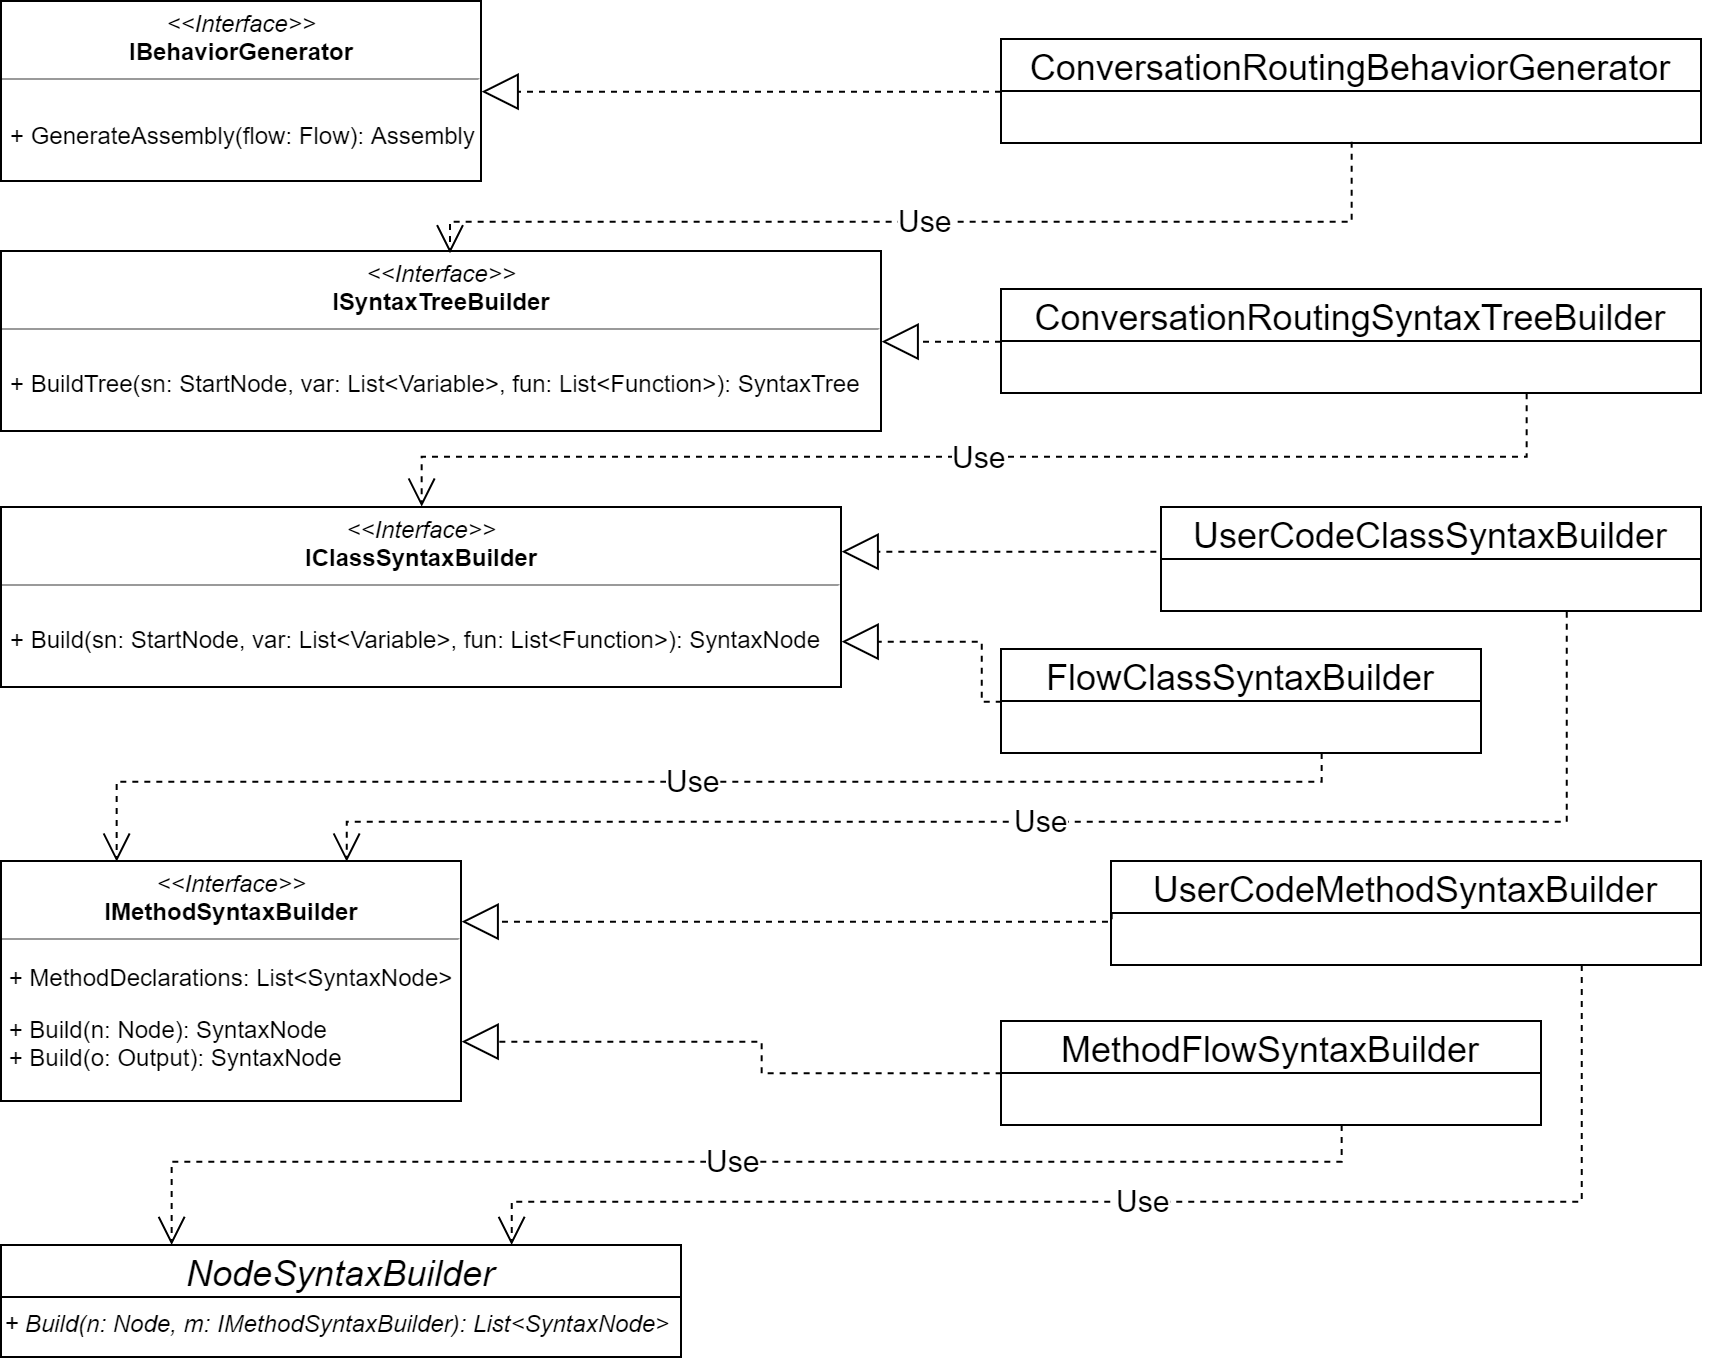
\includegraphics[width=\textwidth]{img/TransformatorUML.png}
	\caption[Klassenstruktur des Transformators]{\textit{Zu sehen ist die Klassenstruktur des Transformators. Die Hauptfunktionalitäten sind in den Interfaces abgebildet. Für die Implementierung dieser Methoden sind wiederum Funktionalitäten notwendig, die in anderen Interfaces definiert sind.}}
	\label{fig:UML:Transformator}
\end{figure}
\noindent Das Hauptelement ist die Klasse \texttt{ConversationRoutingBehaviorGenerator}, welche das Interface \texttt{IBehaviorGenerator} implementiert. Dieses Interface stellt die Methode \texttt{GenerateAssembly} zur Verfügung, welche einen Objekt-Graph in Form einer \texttt{Flow}-Instanz entgegennimmt und eine CIL-Assembly zurückliefert.  Dafür muss der Objekt-Graph jedoch zuerst in einen CIL-Syntaxbaum konvertiert werden. Zum Erstellen dieses Syntaxbaums wird die Methode \texttt{BuildTree} des Interfaces \texttt{ISyntaxTreeBuilder} verwendet, welches von der Klasse \texttt{Con\-ver\-sa\-tion\-Rou\-ting\-Syn\-tax\-Tree\-Buil\-der} implementiert wird. \texttt{BuildTree} nimmt die Instanz vom Typen \texttt{StartNode} des Objekt-Graphen sowie die \texttt{Variable}- und \texttt{Function}-Instanzen entgegen, und liefert einen kompilierbaren Syntaxbaum zurück. Für den Fall einer im Objekt-Graphen vorhandenen \texttt{Vir\-tu\-al\-Start\-Node}-Instanz stellt das Interface auch eine Überladung von \texttt{Build\-Tree} zur Verfügung, welche zusätzlich diese Instanz entgegennimmt. Der Syntaxbaum wird aus kleineren Einheiten zusammengesetzt: Auf der höchsten Ebene stehen die Klassendeklarationen, welche wiederum die Membermethodendeklarationen beinhalten. Wie diese Einheiten generiert werden, wird in den folgenden Abschnitten erläutert.

\subsubsection{Programmablauf}
\label{subsubsec:Programablauf}
Die Grundidee der Syntax-Zusammensetzung orientiert sich an einem Verfahren, das in \cite[S. 272f]{Voelter:13} als ''klassische Modell-Transformierung`` (engl. classical model transformation) bezeichnet wird: Das semantische Modell (hier ein Objekt-Graph) wird als Graph traversiert, während mit der Roslyn-API anhand des aktuell besuchten Objekts die passende Syntax generiert wird. Die Traversierung beginnt bei der Instanz desjenigen \texttt{Node}-Subtyps, der die Start-Instruktion abbildet (\texttt{StartNode}) und besucht jedes Objekt des Objekt-Graphen in der Reihenfolge einer Tiefensuche. Pro besuchtem Objekt wird die CIL-Syntax für eine Methode erstellt, welche das Verhalten derjenigen Instruktion umsetzt, die von dem Objekt abgebildet wird. Dort wo die Syntax die Methode der nachfolgenden Instruktion aufruft, wird das Objekt, welches wiederum diese nachfolgende Instruktion abbildet, rekursiv besucht und dort die entsprechende Syntax für die abbildende Methode erstellt. Dies geht so lange weiter, bis eine Instruktion erreicht wird, die keine ausgehenden Verbindungen hat. An dieser Stelle ist der Rekursionsanker erreicht: Die Syntax für die letzte Instruktion des aktuellen Pfades wird generiert, der Liste der Membermethoden hinzugefügt, und der Aufruf der so generierten Methode an die Vorgänger-Methode zurückgeliefert. Diese kann den erhaltenen Aufruf nun in ihre eigene Syntax integrieren und ihren eigenen Aufruf an die eigene Vorgänger-Instruktion zurückliefern. Der Programmfluss kehrt auf diese Weise zurück zur Start-Instruktion, wo der letzte Methodenaufruf in die Methode \texttt{StartAsync} integriert wird. Zu diesem Zeitpunkt sind alle Methodendeklarationen erstellt und können der Klassendeklaration hinzugefügt werden. Für den Fall, dass im Objekt-Graph eine Instanz des Typs \texttt{VirtualStartNode} vorhanden ist, wird der Vorgang zweimal durchgeführt, da dieser \texttt{Node}-Subtyp genau wie \texttt{StartNode} einen Einstiegspunkt im Konversationsrouting abbildet. Daher muss mit dem gleichen Verfahren eine Methoden-Aufrufkette generiert werden, welche in der Membermethode \texttt{VirtualStartAsync} beginnt.
\newline
Da ein Konversationsrouting Zyklen enthalten kann, muss überprüft werden, ob ein solcher Zyklus im Routing vorhanden ist, um einen Aufrufstapelüberlauf durch die entstehende endlose Rekursion zu vermeiden (siehe \ref{subsec:Konzept}). Daher wird während des rekursiven Ablaufs mit einem Stapelspeicher Protokoll geführt, welche \texttt{Input}-Instanzen des Objekt-Graphen schon besucht wurden. Beim Besuchen einer \texttt{Input}-Instanz wird diese auf den Stapel gelegt, beim Verlassen auf dem Rückweg der Rekursion wird dieser wieder entnommen. Wird eine \texttt{Input}-Instanz besucht, die sich schon auf dem Stapelspeicher befindet, ist die Instanz des \texttt{Node}-Subtypen, die die \texttt{Input}-Instanz beinhaltet, schon besucht worden und die Rekursion kann abgebrochen werden. Der zurückzuliefernde Methoden-Aufruf für diese \texttt{Node}-Subtypen-Instanz wird dann in einem neuen Thread ausgeführt. 
\newline
Die Struktur der Klassen, die den obenstehenden Algorithmus umsetzen, ist in Abbildung \ref{fig:UML:Transformator} zu sehen. Die Klasse \texttt{FlowClassSyntaxBuilder} implementiert die Schnittstelle \texttt{IClassSyntaxBuilder}, welche die Methode \texttt{Build} zur Verfügung stellt. \texttt{Build} nimmt eine Referenz auf die \texttt{StartNode} entgegen und liefert eine Klassendeklaration in Form einer \texttt{SyntaxNode} zurück. \texttt{SyntaxNode} ist ein Typ der Roslyn-API, welcher einen Knoten im CIL-Syntaxbaum repräsentiert. Falls der zu übergebende Objekt-Graph eine Instanz von \texttt{VirtualStartNode} beinhaltet, wird diese in einer Überladung der Build-Methode übergeben, welche ein zusätzliches Argument akzeptiert. \texttt{FlowClassSyntaxBuilder} implementiert \texttt{IFlowClassSyntaxBuilder} indem es die Syntax für die zu generierende Klasse erstellt. Zum Erstellen der Membermethoden der Klasse wird das Interface \texttt{IMethodSyntaxBuilder} benutzt, welches von der Klasse \texttt{Meth\-od\-Flow\-Syn\-tax\-Buil\-der} implementiert wird. \texttt{IMe\-thod\-Syn\-tax\-Buil\-der} stellt Methoden zur Verfügung, welche Instanzen von \texttt{Node} oder \texttt{Output} entgegennehmen und eine Methodendeklaration zurückliefern, welche die übergebene \texttt{Node} abbildet. \texttt{Meth\-od\-Flow\-Syn\-tax\-Buil\-der} implementiert diese Methoden mithilfe des rekursiven Prozesses, der weiter oben erläutert ist. Zu diesem Zweck implementiert die Klasse das Visitor-Pattern in Form des Interfaces \texttt{IFlowNodeVisitor}, in dem Methoden bereit gestellt werden, mit der alle \texttt{Node}-Subtypen sowie Inputs und Outputs besucht werden können (vgl. \cite[S. 5f]{Jones}, wo dieses Verfahren für abstrakte Syntaxbäume empfohlen wird). Bei dem Besuch einer \texttt{Node}-Subtyp-Instanz muss je nach Subtyp bestimmte CIL-Syntax erstellt werden. Zu diesem Zweck existiert die abstrakte Klasse \texttt{NodeSyntaxBuilder}, von der pro \texttt{Node}-Subtyp eine Klasse erbt. Jeder dieser erbenden Klassen generiert die Syntax für den jeweiligen \texttt{Node}-Subtyp, für den sie zuständig ist. Dies geschieht in der überschriebenen \texttt{Build}-Methode der Basisklasse \texttt{NodeSyntaxBuilder}, welche die Syntax an \texttt{MethodFlowSyntaxBuilder} zurückliefert. Der Ablauf ist in den Diagrammen \ref{fig:UML:TransformationSequence} und \ref{fig:UML:TransformationSequenceDetail} abgebildet und wird wie folgt abgewickelt:

\begin{figure} %[hbtp]
	\centering
		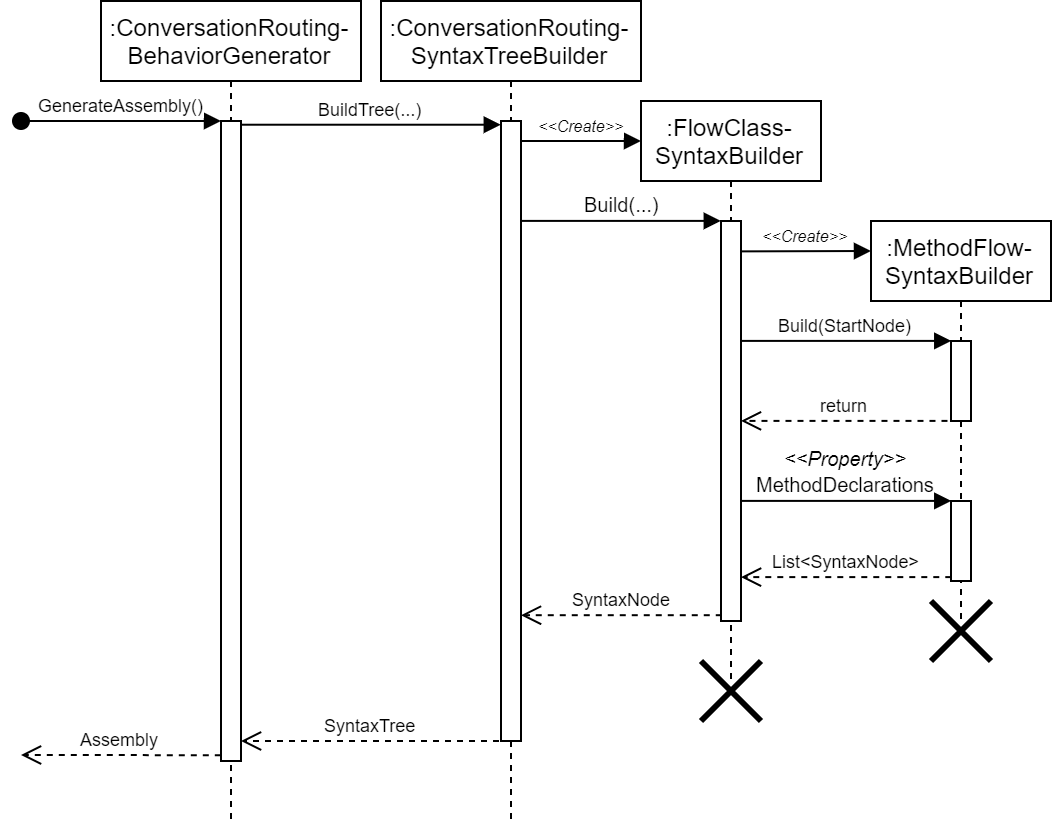
\includegraphics[width=\textwidth]{img/TransformationSequence.png}
	\caption[Transformationsablauf]{\textit{Grober Ablauf der Transformation als Sequenzdiagramm. Für den detailierten Ablauf in \texttt{MethodFlowSyntaxBuilder} siehe Abb. \ref{fig:UML:TransformationSequenceDetail} }}
	\label{fig:UML:TransformationSequence}
\end{figure}

\begin{figure} %[hbtp]
	\centering
		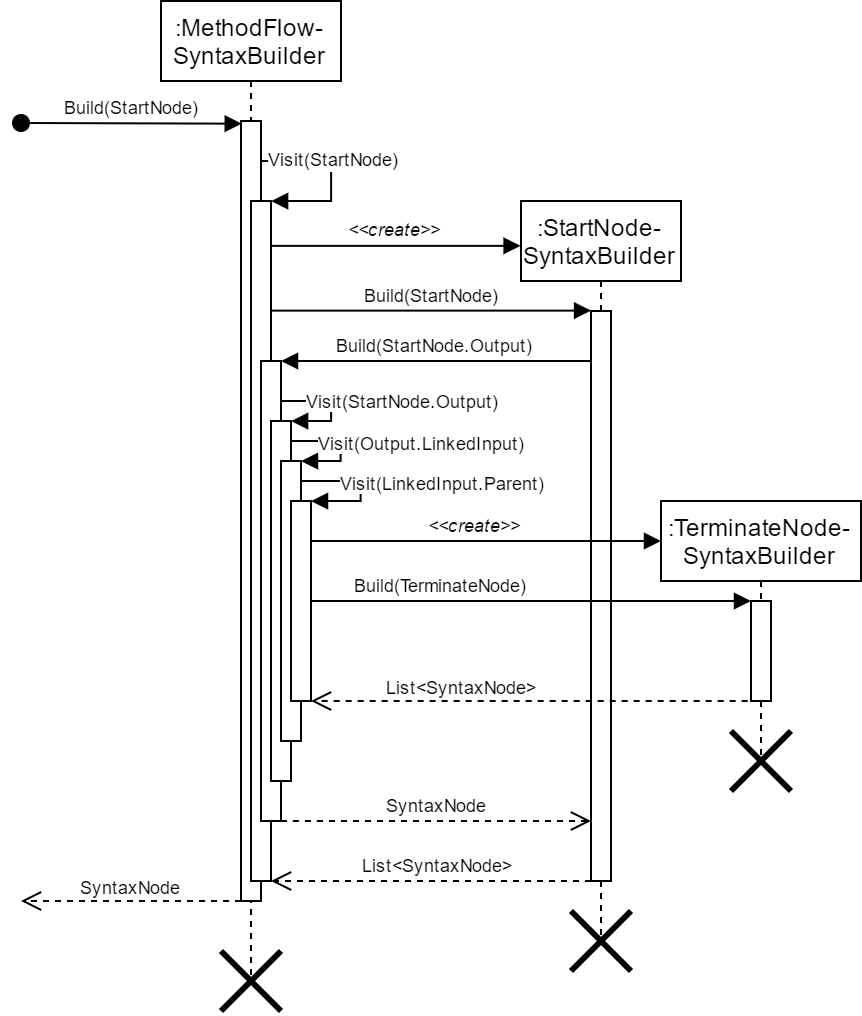
\includegraphics[width=0.8\textwidth]{img/TransformationSequenceDetail.png}
	\caption[Transformationsablauf im Detail]{\textit{Ablauf der Generierung der Methodensyntax im Detail. Zu sehen ist der rekursive Ablauf des Verhaltens der Klasse \texttt{MethodFlowSyntaxBuilder}. In dem abgebildeten Diagramm ist der Ablauf zur Erstellung einer Syntax für ein Konversationsrouting  abgebildet, bei dem die Start-Instruktion direkt in die Terminate-Instruktion mündet. Das Beispiel ist so simpel gehalten, um die Komplexität des Diagramms nicht unnötig zu erhöhen.}}
	\label{fig:UML:TransformationSequenceDetail}
\end{figure}
\noindent Ein Aufruf an die Methode \texttt{GenerateAssembly} der \texttt{Con\-ver\-sa\-tion\-Rou\-ting\-Be\-ha\-vior\-Gen\-era\-tor}-Instanz ruft zum Erstellen des Syntaxbaums die \texttt{Build\-Tree}-Methode auf der \texttt{Con\-ver\-sa\-tion\-Rou\-ting\-Syn\-tax\-Tree\-Buil\-der}-Instanz auf. Diese Klasse instanziert \texttt{Flow\-Class\-Syn\-tax\-Buil\-der}. Hier wird zuerst die \texttt{Build}-Methode für die \texttt{StartNode}-Referenz einer \texttt{Flow}-Instanz aufgerufen, in der eine Instanz von \texttt{StartNodeSyntaxBuilder} erzeugt wird. Auf dieser Instanz wird nun die Methode \texttt{Build} aufgerufen, welcher neben der Referenz auf die \texttt{StartNode}-Instanz auch die aufrufende Instanz von \texttt{Meth\-od\-Flow\-Syn\-tax\-Buil\-der} übergeben wird. So kann \texttt{StartNodeSyntaxBuilder} für die \texttt{Output}-Instanz, die in \texttt{StartNode} enthalten ist, \texttt{MethodFlowSyntaxBuilder.Build} aufrufen, in der wiederum die \texttt{Visit}-Methode aufgerufen wird. In der \texttt{Visit}-Methode wird nun \texttt{Visit} für die Input-Instanz aufgerufen, auf welche die \texttt{Output}-Instanz der \texttt{Start\-Node}-Instanz verweist. Dort wird erneut \texttt{Visit} für die \texttt{Node}-Instanz aufgerufen, auf die wiederum die \texttt{Input}-Instanz verweist. Die Rekursion setzt sich hier fort: Es wird ein \texttt{NodeSyntaxBuilder} für die aktuell besuchte \texttt{Node}-Subtyp-Instanz erstellt und \texttt{Build} aufgerufen. Innerhalb der \texttt{Build}-Methode des \texttt{NodeSyntaxBuilders} wird jetzt die CIL-Syntax für die Instruktion in Form einer Liste von \texttt{SyntaxNode}-Instanzen erstellt. Hat die aktuelle \texttt{Node}-Subtyp-Instanz weitere \texttt{Output}-Instanzen, wird auch hier wieder \texttt{Meth\-od\-Flow\-Syn\-tax\-Buil\-der.Build} für diese aufgerufen. Handelt es sich jedoch um eine Instruktion ohne Ausgänge, ist der Rekursionsanker erreicht. Der aktuelle \texttt{NodeSyntaxBuilder} liefert seine Liste mit \texttt{SyntaxNode}-Instanzen an den \texttt{Meth\-od\-Flow\-Syn\-tax\-Buil\-der.Visit}-Aufruf zurück. Dort werden die \texttt{SyntaxNode}-Instanzen zu einer Methodendeklaration zusammengefasst und gespeichert. Der \texttt{Visit}-Aufruf kehrt zu seinem \texttt{Build}-Aufruf zurück und gibt als Rückgabe-Wert eine \texttt{SyntaxNode}-Instanz zurück, in der ein Aufruf der eben erstellten Methodendeklaration enthalten ist. Dieser Aufruf kehrt zu dem \texttt{Build}-Aufruf von \texttt{StartNodeSyntaxBuilder} zurück, der die Syntax der \texttt{StartNode}-Instanz generiert. Dort kann der Aufruf nun in die Syntax der eigenen Methode integriert werden, welche ihrerseits nun zu \texttt{Me\-thod\-Flow\-Syn\-tax\-Builder} zurückkehrt und der \texttt{StartNode}-Methode hinzugefügt wird. Der Prozess wird für alle Instruktionen eines Konversationsroutings durchgeführt, sodass am Ende die Programmfluss-Struktur aus Abschnitt \ref{subsec:Beispiel} erreicht ist. Falls vorhanden, wird der Vorgang analog für eine Instanz von \texttt{VirtualStartNode} ein zweites Mal durchgeführt.
\newline
\texttt{Meth\-od\-Flow\-Syn\-tax\-Buil\-der} gibt anschließend die Liste der Methodendeklarationen an \texttt{Flow\-Class\-Syn\-tax\-Buil\-der} zurück, welcher eine Klassendeklaration an \texttt{Con\-ver\-sa\-tion\-Rou\-ting\-Syn\-tax\-Tree\-Buil\-der} zurückliefert. Dort wird die Klassendeklaration dem CIL-Syntaxbaum hinzugefügt, welcher anschließend in  \texttt{Con\-ver\-sa\-tion\-Rou\-ting\-Be\-ha\-vior\-Gen\-era\-tor} zu einem Assembly kompiliert wird.

\subsubsection{Asynchrone Methodenausführung}
\label{subsubsec:Nebenlaeufigkeit}
Wie in Abschnitt \ref{sec:Transformation} beschrieben, werden manche Instruktionen auf asynchrone Methoden abgebildet, deren Asynchronität sich durch ein Konversationsrouting ziehen kann. Zum Zeitpunkt der oben beschriebenen Generierung der Pro\-gramm\-ab\-lauf-Syntax muss bekannt sein, welche Instruktionen auf asynchrone Methoden abgebildet werden müssen. Daher wird vor der eigentlichen Generierung ein Vorverarbeitungsschritt ausgeführt, in dem alle Instruktionen des Konversationsroutings gesammelt werden, die auf asynchrone Methoden abgebildet werden müssen. Dafür wird der Objekt-Graph traversiert und \texttt{Node}-Subtyp-Instanzen, welche asynchrone Instruktionen und Instruktionen über die solche erreicht werden können, abbilden, werden in einer Liste vermerkt. Diese Liste wird anschließend \texttt{FlowClassSyntaxBuilder} zur Verfügung gestellt. Die Bestimmung, ob eine \texttt{Node}-Subtyp-Instanz über einen Pfad im Objekt-Graphen eine andere \texttt{Node}-Subtyp-Instanz erreichen kann, welche eine asynchrone Instruktion abbildet, wird über die Berechnung der reflexiv-transitiven Hülle aller \texttt{Node}-Subtyp-Instanzen erreicht. Dies ist eine Liste der direkten und indirekten \texttt{Node}-Subtyp-Vorgänger aller \texttt{Node}-Subtyp-Instanzen im Objekt-Graph. Eine \texttt{Node}-Subtyp-Instanz muss dann zu einer asynchron Methode transformiert werden, wenn ihre zu generierende Methodensyntax eine asynchrone API-Methode aufruft, oder in der reflexiv-transitiven Hülle in Relation mit einer anderen \texttt{Node}-Subtyp-Instanz steht, deren zu generierende Syntax asynchrone Methoden aufruft.

\subsubsection{Benutzerdefinierter Code}
Vom Benutzer spezifizierter Code wird in einer generierten Klasse namens \texttt{UserCode} gekapselt. Die Syntax für die Deklaration dieser Klasse wird von einer weiteren Implementierung des Interfaces \texttt{IClassSyntaxBuilder} namens \texttt{User\-Code\-Class\-Syn\-tax\-Buil\-der} übernommen. Da die \texttt{UserCode}-Klasse eine private Klasse ist, muss ihre Deklaration der Syntax für die Routing-steuernde Klasse hinzugefügt werden. Daher wird \texttt{UserCodeClassSyntaxBuilder} von \texttt{FlowClassSyntaxBuilder} benutzt. Die beiden Klassen ähneln sich in der Art und Weise, wie sie die Syntax für die jeweils eigene Klassendeklaration generieren: \texttt{UserCodeClassSyntaxBuilder} verwendet den gleichen rekursiven Ablauf zur Traversierung des Objekt-Graphen wie in Abschnitt \ref{subsubsec:Programablauf} beschrieben, nur dass dieser in seiner eigenen Klasse namens \texttt{UserCodeMethodSyntaxBuilder} implementiert ist. \texttt{User\-Code\-Meth\-od\-Syn\-tax\-Buil\-der} behandelt beim Besuchen der Instruktionen nur \texttt{Node}-Subtypen, in denen benutzerspezifizierter Code zu finden ist. Für diese Subtypen werden bestimmte \texttt{NodeSyntaxBuilder}-Subtypen instanziert, welche den Code des Benutzers parsen und in die zu erstellenden Methodendeklarationen der \texttt{UserCode}-Klasse einbetten. Außerdem bearbeitet \texttt{UserCodeClassSyntaxBuilder} auch die benutzerdefinierten Variablen und Funktionen. Diese werden der Reihe nach durchgegangen und die entsprechend generierte Syntax in Form von Methoden- und Variablendeklarationen wird der Klasse \texttt{UserCode} hinzugefügt. Die so entstehende \texttt{UserCode}-Klassendeklaration wird an \texttt{FlowClassSyntaxBuilder} übergeben, wo sie als private geschachtelte Klassendeklaration in die umfassende Klasse eingebettet wird.

\section{Modell-Validierung} 
Eine Aufgabe der DSL ist die Unterstützung des Benutzers, indem Fehler vermieden oder schnell beseitigt werden. Dafür ist es von hoher Bedeutung, dem Benutzer Fehlerzustände in einem Konversationsrouting frühzeitig anzuzeigen, damit diese nicht bei der weiteren Modellierung oder Transformation fortbestehen oder sich sogar vervielfachen. Zu diesem Zweck wird während der Modellierung im Editor eine Modell-Validierung durchgeführt, bei der sogenannte Constraints überprüft werden. Bei Constraints handelt es sich laut \cite[S. 82ff, 289ff]{Voelter:13} um Einschränkungen für die Gültigkeit eines DSL-Modells, welche dabei helfen, Fehler vor der endgültigen Transformation zu ermitteln. Daher wird nach jeder Benutzer-Aktion, die das Konversationsrouting verändert, das aktuelle DSL-Modell analysiert und verschiedenen Prüfungen unterzogen. Diese Prüfungen stellen sicher, dass alle Constraints eingehalten werden und zeigen dem Benutzer im Falle eines Verstoßes eine entsprechende Fehlermeldung an.
\newline
Die Modell-Validierung findet im Editor statt. Dort steht dem ViewModel eine Instanz des Interfaces \texttt{IFlowValidator} zur Verfügung, dessen Klassenstruktur im Diagramm \ref{fig:UML:FlowValidatorClassStructure} abgebildet ist.

\begin{figure} %[hbtp]
	\centering
		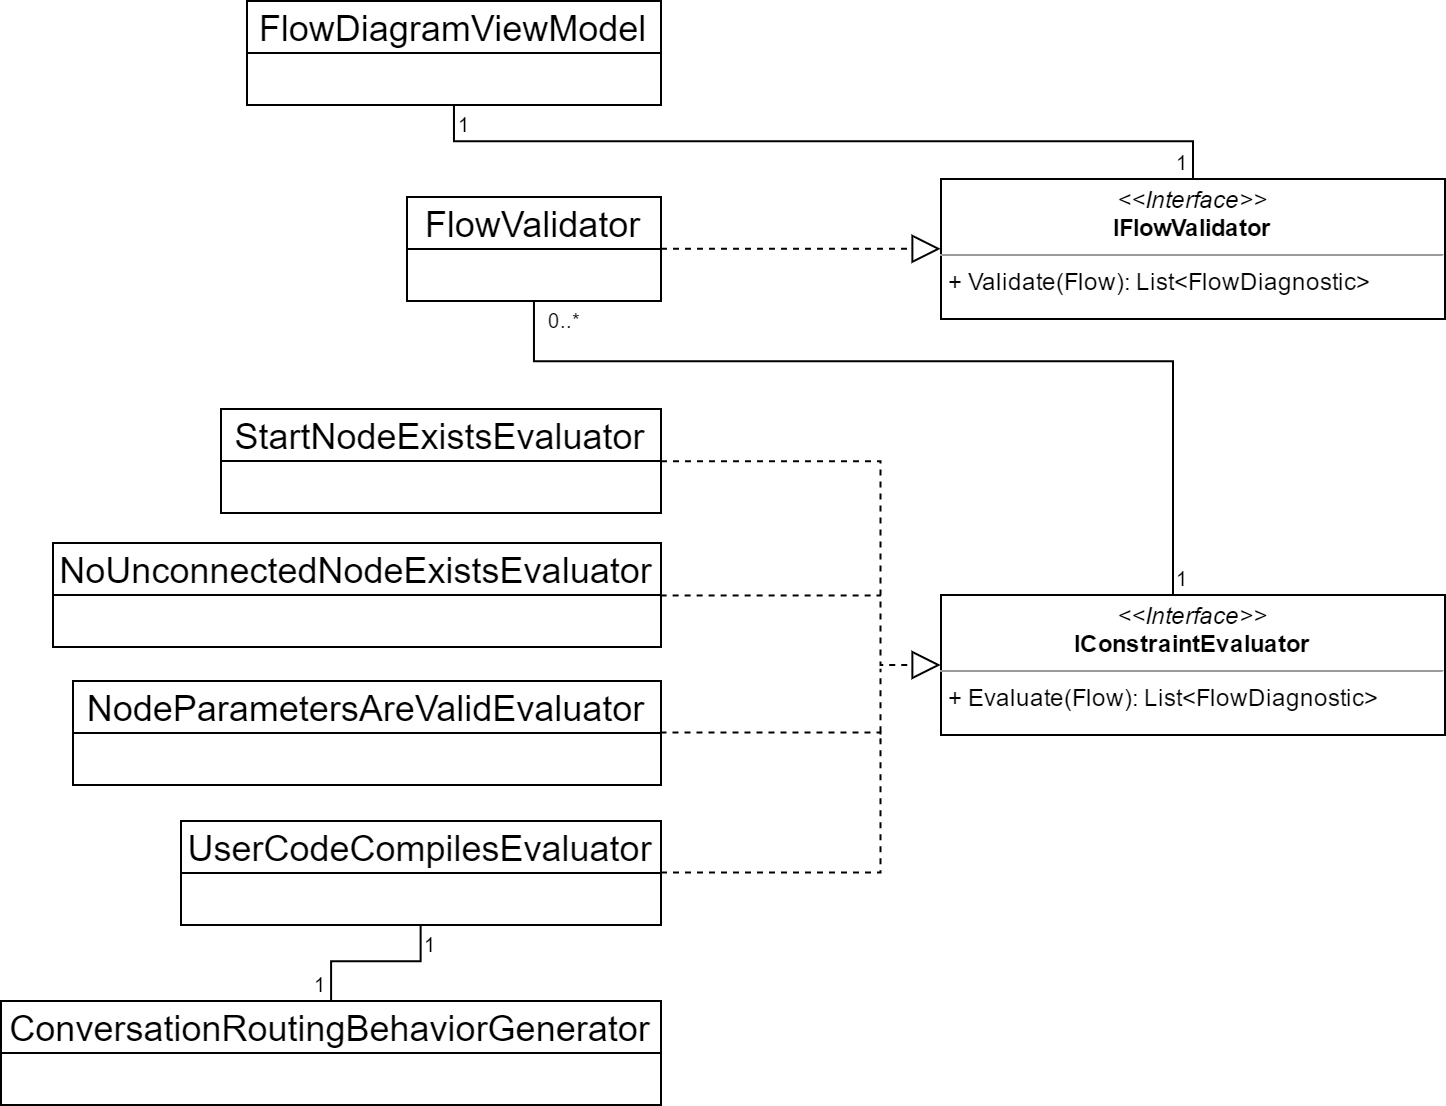
\includegraphics[width=\textwidth]{img/FlowValidatorClassStructure.png}
	\caption[Klassenstruktur der Modell-Validierung]{\textit{Abgebildet ist die Klassenstruktur der Modell-Validierung. Die Klasse \texttt{FlowValidator} benutzt eine Reihe von \texttt{IConstraintEvaluator}-Instanzen, um die etwaige Constraint-Verstöße eines Modells als eine Liste von \texttt{FlowDiagnostic}-Instanzen an das ViewModel weiterzuleiten.}}
	\label{fig:UML:FlowValidatorClassStructure}
\end{figure}
\noindent Die Klasse \texttt{FlowValidator} implementiert \texttt{IFlowValidator}, welche die Methode \texttt{Validate} zur Verfügung stellt. \texttt{Validate} nimmt ein semantisches Modell in Form einer \texttt{Flow}-Instanz entgegen und liefert eine Liste von \texttt{FlowDiagnostics} zurück, in denen Details zu auftretenden Fehlern wie zum Beispiel eine Fehlernachricht oder die betroffene Instruktion gespeichert sind. Zur Implementierung des Interfaces benutzt \texttt{FlowValidator} eine Liste von Klasseninstanzen, die das Interface \texttt{IConstraintEvaluator} implementieren. Diese Interface stellt die Methode \texttt{Evaluate} bereit. \texttt{Evaluate} nimmt eine \texttt{Flow}-Instanz entgegen und überprüft diese auf einen einzelnen Constraint. Verletzt das semantische Modell diesen Constraint, liefert \texttt{Evaluate} eine Liste mit \texttt{FlowDiagnostic}-Instanzen zurück. In der vorliegenden Implementierung sind vier \texttt{ConstraintEvaluator} implementierende Klassen umgesetzt: 
\begin{description}
\item[\texttt{StartNodeExistsEvaluator}] \hfill \\
Diese Implementierung von \texttt{IConstraintEvaluator} überprüft, ob im semantischen Modell eine einzelne Start-Instruktion vorhanden ist.
\item[\texttt{NoUnconnectedNodeExistsEvaluator}] \hfill \\
Hier wird überprüft, ob Instruktionen existieren, deren Eingang mit dem Rest des Konversationsroutings unverbunden ist. Für jede unverbundene Instruktion wird eine Instanz von \texttt{FlowDiagnostic} zurückgeliefert, in der die entsprechenden \texttt{Node}-Subtyp-Instanzen referenziert sind.
\item[\texttt{NodeParametersAreValidEvaluator}] \hfill \\
\texttt{NodeParametersAreValidEvaluator} überprüft, ob die Parameter von allen Instruktionen zulässig sind. So dürfen zum Beispiel für Media Playback-Instruktionen die angegebenen Audio-Dateien nicht null sein. Verstößt eine Instruktion gegen Constraints dieser Art, wird die abbildende \texttt{Node}-Subtyp-Instanz in der zurückgelieferten Liste der \texttt{FlowDiagnostics} mit einer entsprechenden Warnung referenziert.
\item[\texttt{UserCodeCompilesEvaluator}] \hfill \\
\texttt{UserCodeCompilesEvaluator} prüft, ob der vom Benutzer geschriebene Code valide ist und kompiliert. Dafür muss das gesamte DSL-Modell transformiert und kompiliert werden. Daher besitzt \texttt{UserCodeCompilesEvaluator} eine Referenz auf eine \texttt{ConversationRoutingBehaviorGenerator}-Instanz, mit der bei jedem Aufruf von \texttt{Evaluate} das übergebene Modell transformiert wird. Statt einer Assembly wird von der Generator-Instanz allerdings das von Roslyn bereitgestellte semantische Modell der entstehenden CIL-Syntax angefordert. In diesem Objekt speichert die Rosyln-API unter anderem alle Diagnostiken zur generierten Syntax. Existieren solche Diagnostiken nach der Modell-Transformation, werden diese von der Evaluate Funktion in \texttt{FlowDiagnostic}-Instanzen umgewandelt und zurück geliefert.
\end{description}
Wird in der \texttt{FlowViewModel}-Instanz des Editors nun eine Aktion des Benutzers registriert, wird \texttt{FlowValidator.Validate} aufgerufen. Dort wird auf allen Instanzen von \texttt{IConstraintEvaluator} die \texttt{Evaluate}-Methode aufgerufen, die zurückgelieferten \texttt{FlowDiagnostic}-Instanzen gesammelt, und diese anschließend zurückgeliefert. In \texttt{FlowViewModel} werden die \texttt{FlowDiagnostic}-Instanzen nun in einer Liste gespeichert, die per Datenbindung an die View-Schicht gebunden ist. Die \texttt{FlowDiagnostic}-Instanzen werden in einer List-Control angezeigt, welche die Diagnostiken in Form einer Fehlermeldung visualisiert und bei einem Mausklick auf die betroffene Instruktion verweist. Zwischen \texttt{FlowDiagramViewModel} und \texttt{Code\-Edi\-tor\-View\-Mo\-del} werden die \texttt{FlowDiagnostic}-Instanzen mit einem Nachrichten-Service ausgetauscht, der vom Devexpress-Framework angeboten wird. \texttt{Code\-Edi\-tor\-View\-Mo\-del} kann so die Diagnostiken in einer eigenen Liste anzeigen und die Fehler herausfiltern, die nicht den vom Benutzer geschriebenen Code betreffen. Zusätzlich können Fehler so im Code des Benutzers rot unterstrichen werden.